\documentclass[8pt]{beamer}

\newif\ifplacelogo % create a new conditional
\placelogotrue % set it to true

\usetheme{Warsaw}
\usecolortheme{rose}
\usepackage{multicol}
\usepackage{epstopdf}
\usepackage[italic]{hepnames}
\usepackage{tikz}
\usepackage{listings}
\usepackage{times}
\usepackage{amsmath}
\usepackage{verbatim}
\usepackage{hyperref}
\usepackage{bbding}
\lstset{breakatwhitespace,
language=C++,
columns=fullflexible,
keepspaces,
breaklines,
tabsize=3, 
showstringspaces=false,
extendedchars=true}

% TikZ includes!!!
\usepackage{tikz}
\usetikzlibrary{backgrounds}
\usetikzlibrary{calc}
\tikzstyle{every picture}+=[remember picture]
\input{/home/oviazlo/Desktop/beamerPresentations/myReports/latexHelpScripts/tikzGrid.tex}


\begin{document}

% custom colors
\definecolor{olive}{rgb}{0.3, 0.4, .1}
\definecolor{fore}{RGB}{249,242,215}
\definecolor{back}{RGB}{51,51,51}
\definecolor{title}{RGB}{255,0,90}
\definecolor{dgreen}{rgb}{0.,0.6,0.}
\definecolor{gold}{rgb}{1.,0.84,0.}
\definecolor{JungleGreen}{cmyk}{0.99,0,0.52,0}
\definecolor{BlueGreen}{cmyk}{0.85,0,0.33,0}
\definecolor{RawSienna}{cmyk}{0,0.72,1,0.45}
\definecolor{Magenta}{cmyk}{0,1,0,0}

\definecolor{PixelColor}{RGB}{207,232,139}
\definecolor{SCTColor}{RGB}{167,166,255}
\definecolor{TRTColor}{RGB}{250,224,140}
\definecolor{grayColor}{RGB}{153,153,153}

\newcommand{\yRefPosOne}{0.0}
\newcommand{\xRefPosOne}{0.0}
\newcommand{\yRefPosTwo}{0.0}
\newcommand{\xRefPosTwo}{0.0}
\newcommand{\yRefIncrementOne}{0.0}
\newcommand{\xRefIncrementOne}{0.0}
\newcommand{\yRefIncrementTwo}{0.0}
\newcommand{\xRefIncrementTwo}{0.0}

\graphicspath{ {/home/oviazlo/Desktop/beamerPresentations/FCCee/pictures/} }
\DeclareGraphicsExtensions{.eps, .pdf, .png}

\newcommand{\myBox}[2][pink] {
    \noindent\colorbox{#1}{
	\textbf{#2}
    }\par
}

% For nice block (provided by Oleh)
\tikzstyle{mybox} = [draw=red, fill=blue!1, very thick,
    rectangle, rounded corners, inner sep=5pt, inner ysep=9pt]
    
\tikzstyle{PixelBox} = [draw=PixelColor, fill=blue!1, very thick,
    rectangle, rounded corners, inner sep=5pt, inner ysep=9pt]
\tikzstyle{SCTBox} = [draw=SCTColor, fill=blue!1, very thick,
    rectangle, rounded corners, inner sep=5pt, inner ysep=9pt]
\tikzstyle{TRTBox} = [draw=TRTColor, fill=blue!1, very thick,
    rectangle, rounded corners, inner sep=5pt, inner ysep=9pt]

% poster advertisement
\newcommand{\myCenterBox}[2][pink] {
   {\centering
    \noindent\colorbox{#1}{
	\textbf{#2}
    }\par
  }
}

\newcommand{\mySmallCenterBox}[2][pink] {
   {\centering
    \noindent\colorbox{#1}{
	\textbf{{\small #2}}
    }\par
  }
}

\newcommand{\myVerySmallCenterBox}[2][pink] {
   {\centering
    \noindent\colorbox{#1}{
	\textbf{{\scriptsize #2}}
    }\par
  }
}

\newcommand{\backupbegin}{
   \newcounter{finalframe}
   \setcounter{finalframe}{\value{framenumber}}
}
\newcommand{\backupend}{
   \setcounter{framenumber}{\value{finalframe}}
}

\newcommand{\myNode}{\tikz[baseline,inner sep=1pt] \node[anchor=base]}

\definecolor{light-gray}{gray}{0.95}
% poster advertisement


\title[ CLIC-inspired detector for FCC-ee \hspace{13.5em}\insertframenumber/
\inserttotalframenumber]{ Tracking with the CLIC-inspired detector for FCC-ee }


	\author[Oleksandr Viazlo, Emilia Leogrande]{Oleksandr Viazlo, Emilia Leogrande \\ 
% 	{\small ???}
	}
	\institute{\small CERN\\} 
	
       
	\date{31 July 2017}

% 	\logo{ \ifplacelogo \includegraphics[height=1.8cm]{./ID_week2/lund_uni-logo_s.pdf} \hspace{0.4cm} \fi}

	
   	\frame{\titlepage}

   	

\placelogofalse

%*****************************************************************************
\begin{frame}{\large \large Introduction}
 
 \begin{itemize}
  \item This talk covers an update on the CLIC-inspired detector for FCC-ee
  \item An overview of the CLIC detector together with the layout of the detector for FCC-ee has been shown by Emilia in a previous Detector Design meeting
  \item The main focus of this presentation is the layout of the VTX and Tracker subsystems and the overall tracking performance
%   \item TODO PICT: CLIC det and FCCee det
 \end{itemize}

 
\end{frame}
%*****************************************************************************

%*****************************************************************************
\begin{frame}{\large \large CLIC detector}

\renewcommand{\yRefPosOne}{0}
\renewcommand{\xRefPosOne}{5.3}
\renewcommand{\xRefIncrementOne}{5.5}
\begin{tikzpicture}[overlay]

 \node[inner sep=0pt] (tmp) at (\xRefPosOne-2.5,\yRefPosOne-0.5)
    {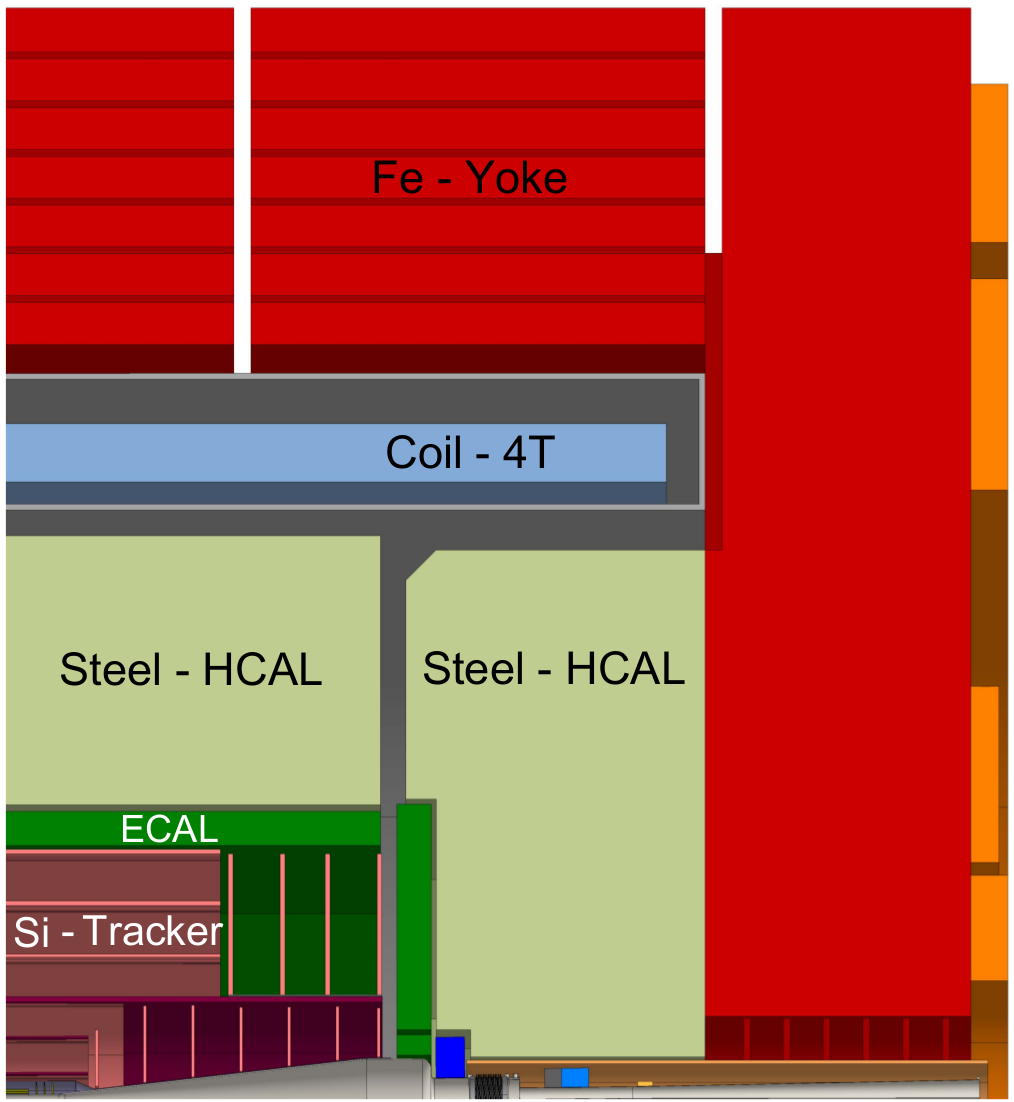
\includegraphics[width=7cm]{CLICdet.png}};

    
\node [Box] at (\xRefPosOne+3.5,\yRefPosOne+1.3) (box){%
    \begin{minipage}{0.5\textwidth}

  \begin{itemize}
   \item Full silicon VTX and Tracker: \\ $\geqslant$12 hits per track
   \item W-Si ECAL and Fe-Scint HCAL
   \item Coil is outside of the calorimeter; \\4 Tesla magnetic field
   \item Steel return yoke with 6 RPC muon chambers
  \end{itemize}

    \end{minipage}
};
% \node[fancytitle, right=15pt] at (box.north west) {Subdetectors};
\node [Box] at (\xRefPosOne+3.5,\yRefPosOne+3.2) (box){%
\myCenterBox{Subdetectors}
};


\node [Box] at (\xRefPosOne+3.5,\yRefPosOne-3) (box){%
    \begin{minipage}{0.5\textwidth}

  \begin{itemize}
   \item Momentum resolution (at 500 GeV): $\sigma_{\mathrm{p_T}}/ \mathrm{p_T}^2 \simeq 2\cdot10^{-5}$ GeV$^{-1}$
   \item Lepton ID efficiency: $>$ 95$\%$
   \item Impact parameter resolution: \\
	 $\sigma_{d_0} = a \oplus \dfrac{b}{p~sin^{3/2} \theta}$ \\ $a \leqslant $5$ \mu$m, $b \leqslant $15 $\mu$m GeV
   \item Jet energy resolution: \\
	 $\sigma_E / E \simeq $ 3.5 $\%$
 \end{itemize}

    \end{minipage}
};

\node [Box] at (\xRefPosOne+3.5,\yRefPosOne-0.9) (box){%
\myCenterBox{Detector requirements}
};


\node [Box] at (\xRefPosOne-0.15,\yRefPosOne+2.9) (box){%
\myCenterBox{CLIC}
};

% \node[fancytitle, right=15pt] at (box.north west) {Detector requirements};

%% HELPER draw advanced helping grid with axises:
% \draw(-0.5,-4) to[grid with coordinates] (11.5,4);
\end{tikzpicture}

 
\end{frame}
%*****************************************************************************

%*****************************************************************************
\begin{frame}{\large \large FCC-ee detector model}
 
\renewcommand{\yRefPosOne}{0}
\renewcommand{\xRefPosOne}{5.3}
\renewcommand{\xRefIncrementOne}{5.5}
\begin{tikzpicture}[overlay]

\node [Box] at (\xRefPosOne,\yRefPosOne) (box){%
    \begin{minipage}{0.99\textwidth}
      \begin{itemize}
      %   \item First implementation of the FCCee detector model was based on CLIC$\_$o2$\_$v4 model.
	\item Latest version of the detector, FCCee$\_$o5$\_$v03, is based on the latest CLIC model (CLIC$\_$o3$\_$v12), 
	      which makes it compatible with the latest ILCSoft and CLIC subdetector drivers.
	\item All future bug-fixes of drivers and updates of algorithms will work for both CLIC and FCC-ee models.
	\item Intensive testing and verification of the detector model were done to make sure that simulation and reconstruction work as expected.
      \end{itemize}
    \end{minipage}
};


%  \node[TRTBox] (tmp) at (\xRefPosOne-3,\yRefPosOne-2.5)
%   { 
%     \begin{minipage}{0.5\textwidth}
% 
%     \resizebox{\columnwidth}{!}{%
%       \begin{tabular}{lccc}
% 	 & CLIC & & FCC-ee \\[0.18cm]
% 	VTX Barrel & 31-60 mm & $\Longrightarrow$ & 17-59 mm \\[0.18cm]
% 	VTX Endcap & Spirals & $\Longrightarrow$ & Disks \\[0.18cm]
% 	Tracker Radius & 1486 mm & $\Longrightarrow$ & 2100 mm \\[0.18cm]
%       \end{tabular}%
%     }
%     \end{minipage}
%   };
%   
%  \node[TRTBox] (tmp) at (\xRefPosOne+3.2,\yRefPosOne-2.5)
%   { 
%     \begin{minipage}{0.54\textwidth}
% 
%     \resizebox{\columnwidth}{!}{%
%       \begin{tabular}{lccc}
% 	 & CLIC & & FCC-ee \\[0.18cm]
% 	ECAL thickness & 202 mm & $\Longrightarrow$ & 202 mm \\[0.18cm]
% 	HCAL thickness & 44 $\times$ 7.5 $\lambda_0$ & $\Longrightarrow$ & 44 $\times$ 5.5 $\lambda_0$ \\[0.18cm]
% 	Yoke Thickness & 1989 mm & $\Longrightarrow$ & 1521 mm \\[0.18cm]
%       \end{tabular}%
%     }
%     \end{minipage}
%   };
% 
% \node [Box] at (\xRefPosOne,\yRefPosOne-1) (box){%
% \myCenterBox{Overall dimensions of CLIC and FCC-ee detectors}
% };
  
\end{tikzpicture}
\end{frame}
%*****************************************************************************

%*****************************************************************************
\begin{frame}{\large \large FCC-ee detector}
 
\renewcommand{\yRefPosOne}{0}
\renewcommand{\xRefPosOne}{5.3}
\renewcommand{\xRefIncrementOne}{5.5}
\begin{tikzpicture}[overlay]


 \node[TRTBox] (tmp) at (\xRefPosOne,\yRefPosOne-0.5)
  { 
    \begin{minipage}{0.8\textwidth}

    \resizebox{\columnwidth}{!}{%
      \begin{tabular}{lccc}
	 & CLIC & & FCC-ee \\[0.18cm]
	VTX Barrel & 31-60 mm & $\Longrightarrow$ & 17-59 mm \\[0.18cm]
	VTX Endcap & Spirals & $\Longrightarrow$ & Disks \\[0.18cm]
	Tracker radius & 1486 mm & $\Longrightarrow$ & 2100 mm \\[0.18cm]
% 	ECAL thickness & 202 mm & $\Longrightarrow$ & 202 mm \\[0.18cm]
% 	HCAL thickness & 44 $\times$ 7.5 $\lambda_0$ & $\Longrightarrow$ & 44 $\times$ 5.5 $\lambda_0$ \\[0.18cm]
	ECAL thickness & 40 layers, 22 X$_0$ & $\Longrightarrow$ & 40 layers, 22 X$_0$ \\[0.18cm]
	HCAL thickness & 60 layers, 7.5 $\lambda_I$ & $\Longrightarrow$ & 44 layers, 5.5 $\lambda_I$ \\[0.18cm]
	Yoke thickness & 1989 mm & $\Longrightarrow$ & 1521 mm \\[0.18cm]
	MDI (forward region) &  & $\Longrightarrow$ & $<$ 150 mrad \\[0.4cm]
	Solenoid field & 4 Tesla & $\Longrightarrow$ & 2 Tesla \\
	
      \end{tabular}%
    }
    \end{minipage}
  };
  


\node [Box] at (\xRefPosOne,\yRefPosOne+2.6) (box){%
\myCenterBox[TRTColor]{Overall dimensions of CLIC and FCC-ee detectors}
};
  
\end{tikzpicture}
\end{frame}
%*****************************************************************************

%*****************************************************************************
\begin{frame}{\large \large VTX and Tracker layout}
 
\renewcommand{\yRefPosOne}{0}
\renewcommand{\xRefPosOne}{5.3}
\renewcommand{\xRefIncrementOne}{5.5}
\begin{tikzpicture}[overlay]

%  \node[inner sep=0pt] (tmp) at (\xRefPosOne,\yRefPosOne-1.9)
%     {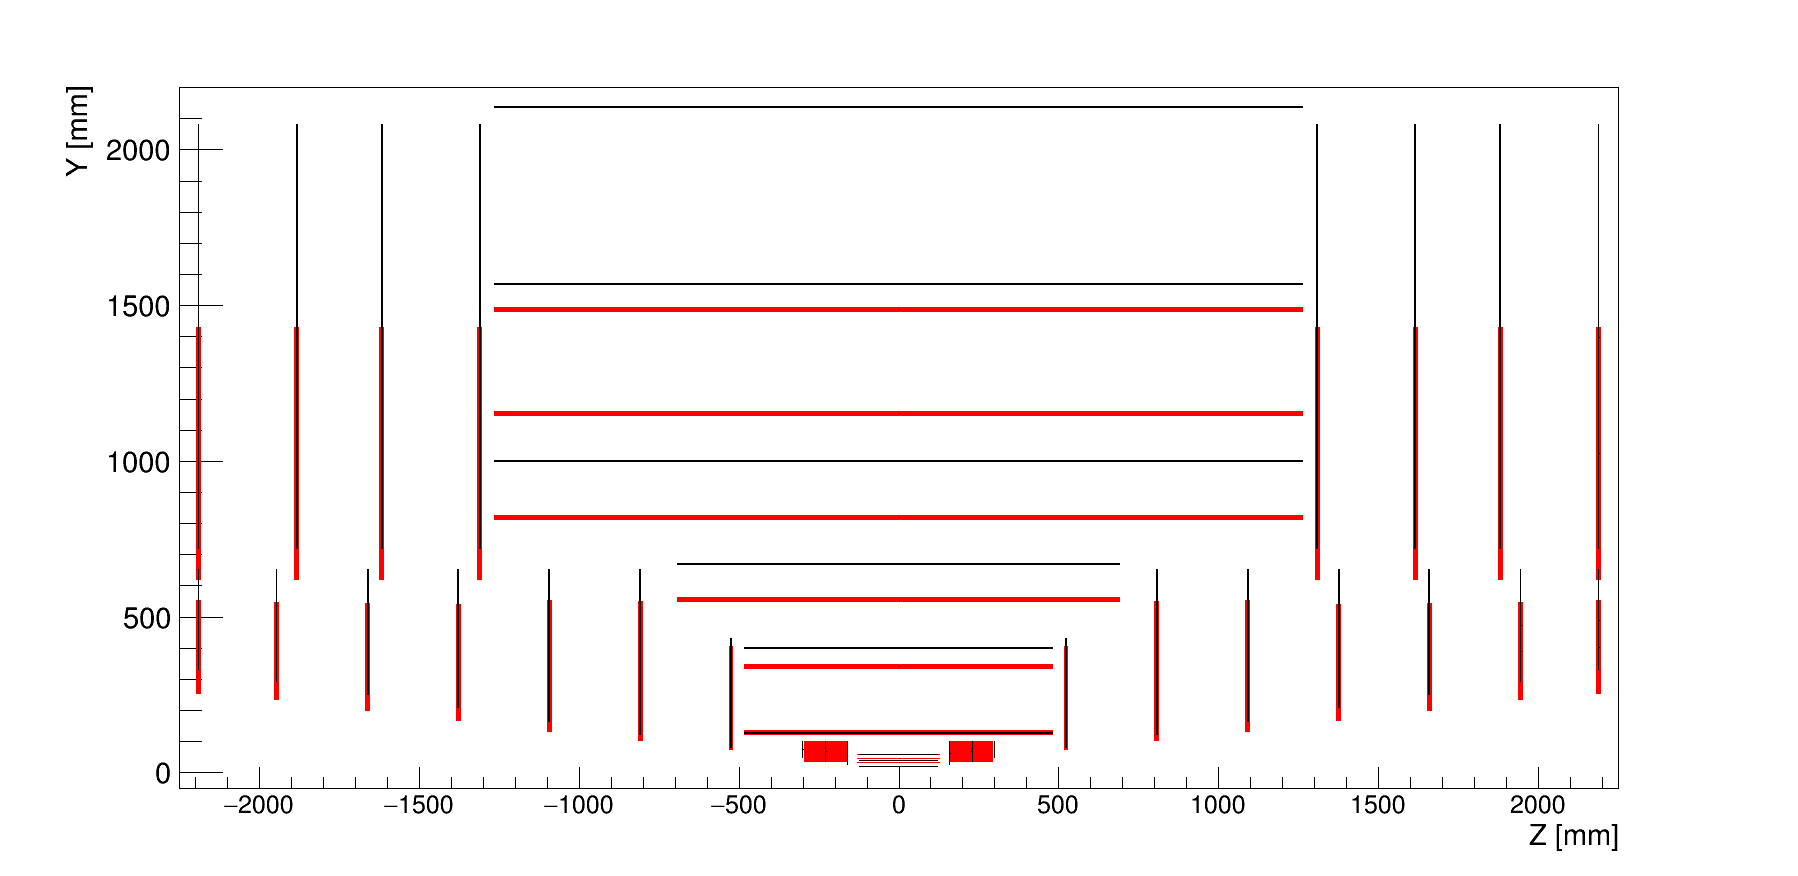
\includegraphics[width=12cm]{CLIC_vs_FCCee_trackingSystem.png}};

    
\node [Box] at (\xRefPosOne,\yRefPosOne+2) (box){%
    \begin{minipage}{0.99\textwidth}

      \begin{itemize}
  \item Overall structure of VTX and Tracker is the same as in the CLIC detector
  \item VTX barrel is a scaled version of the CLIC VTX barrel
%   provides the best coverage and homogenity in number of hits as function of theta
  \item VTX endcaps consists of disks (while CLIC has spirals, to allow air cooling)
  \item Tracker radius is increased to compensate for smaller magnetic field
  \item Minimum radius of the IT disks is adjusted to the MDI region, 150 mrad
      \end{itemize}

    \end{minipage}
};
% \node[fancytitle, right=15pt] at (box.north west) {Transition Radiation Tracker};

 \node[inner sep=0pt] (tmp) at (\xRefPosOne,\yRefPosOne-2.2)
%     {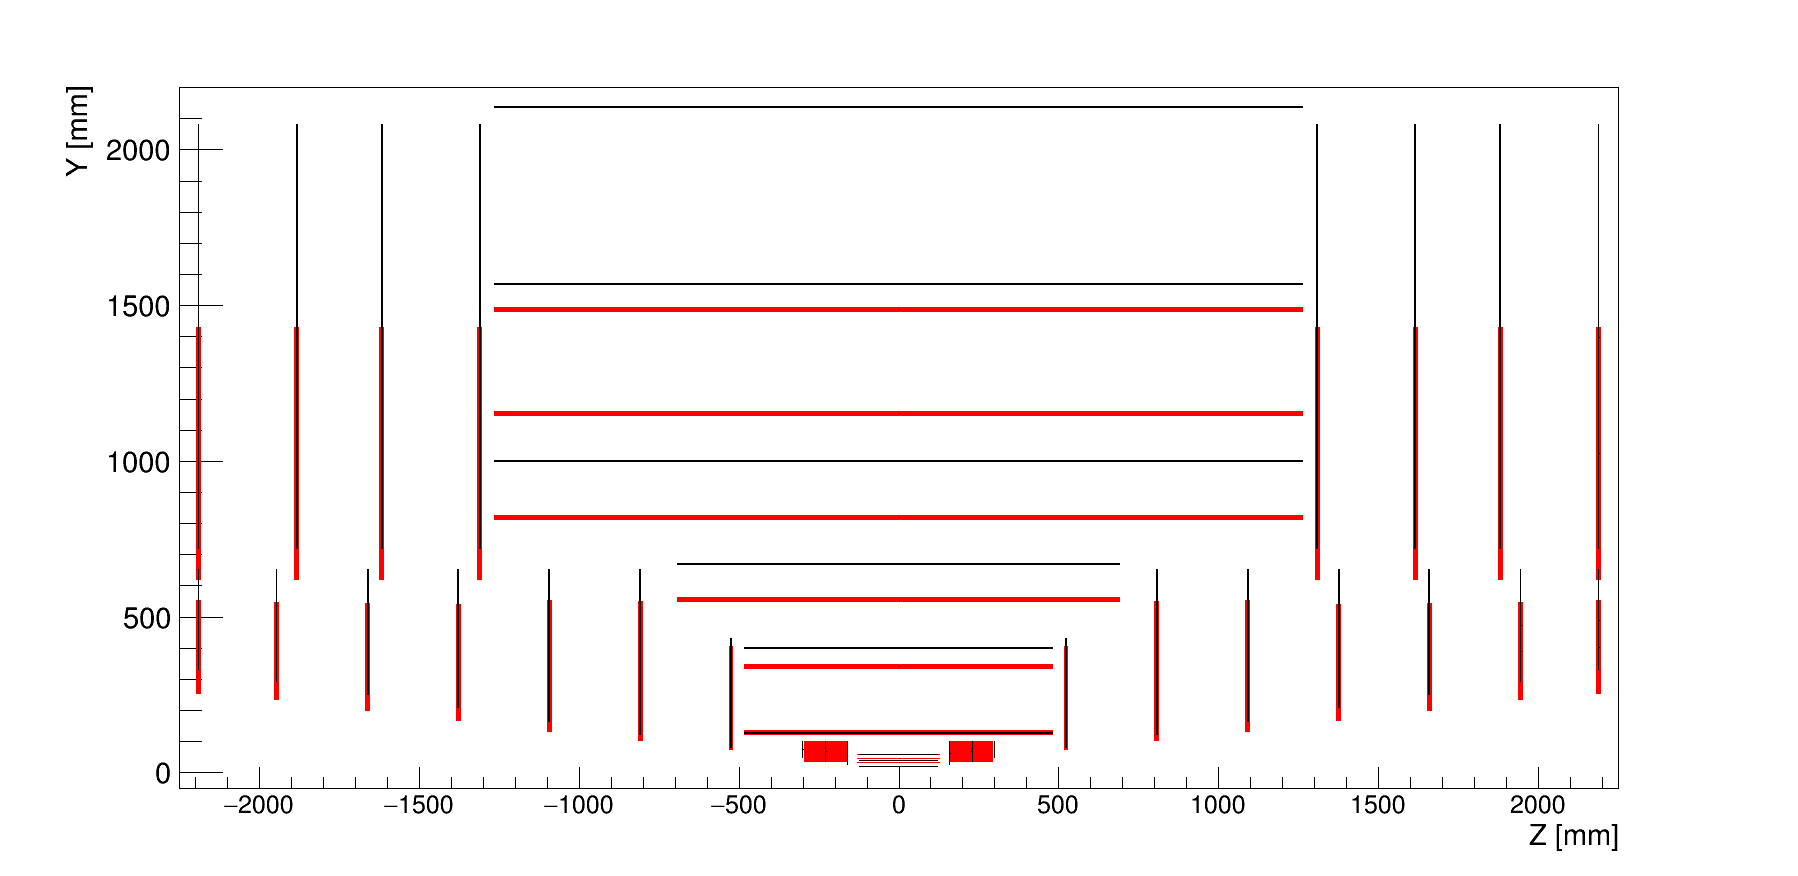
\includegraphics[width=12cm]{CLIC_vs_FCCee_trackingSystem.png}};
  {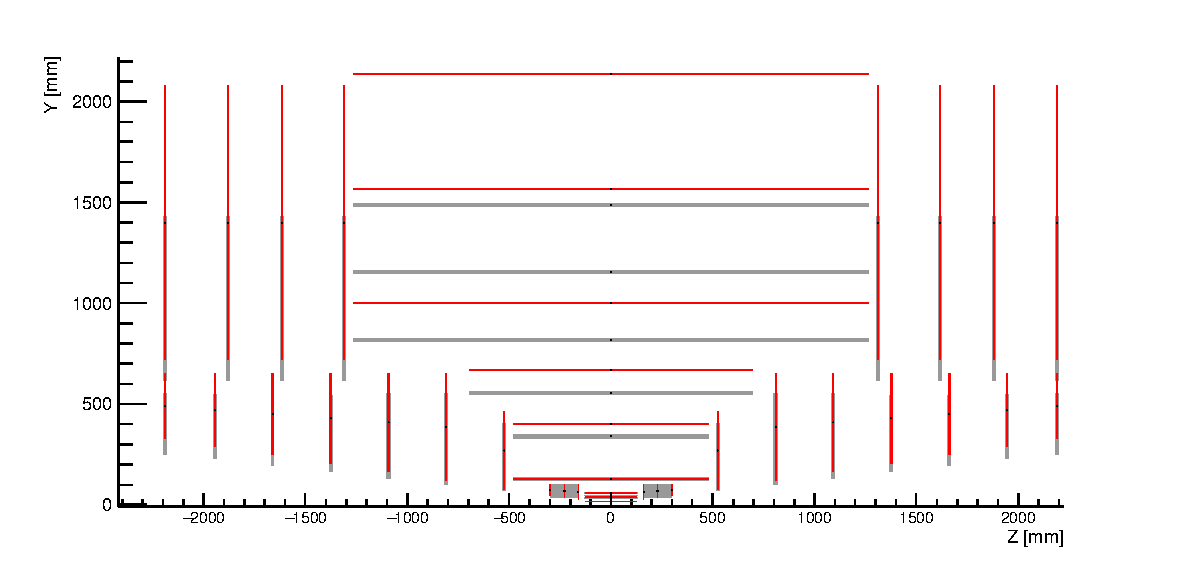
\includegraphics[width=12cm]{geometryComparison_v3.pdf}};


\node [Box] at (\xRefPosOne,\yRefPosOne+0.4) (box){%
\myCenterBox{Comparison of the CLIC and FCC-ee tracking system}
};
    
\node [Box] at (\xRefPosOne+5.35,\yRefPosOne-1.8) (box){%
\myVerySmallCenterBox[grayColor]{CLIC}
};
    
\node [Box] at (\xRefPosOne+5.35,\yRefPosOne-2.5) (box){%
\myVerySmallCenterBox[red]{FCC-ee}
};
    
%% HELPER draw advanced helping grid with axises:
% \draw(-0.5,-4) to[grid with coordinates] (11.5,4);
\end{tikzpicture}

  
\end{frame}
%*****************************************************************************

%*****************************************************************************
\begin{frame}{\large \large Coverage of VTX and Tracker detectors}
 
 
\renewcommand{\yRefPosOne}{0}
\renewcommand{\xRefPosOne}{5.3}
\renewcommand{\xRefIncrementOne}{5.5}
\begin{tikzpicture}[overlay]

%  \node[inner sep=0pt] (tmp) at (\xRefPosOne,\yRefPosOne-2.5)
%     {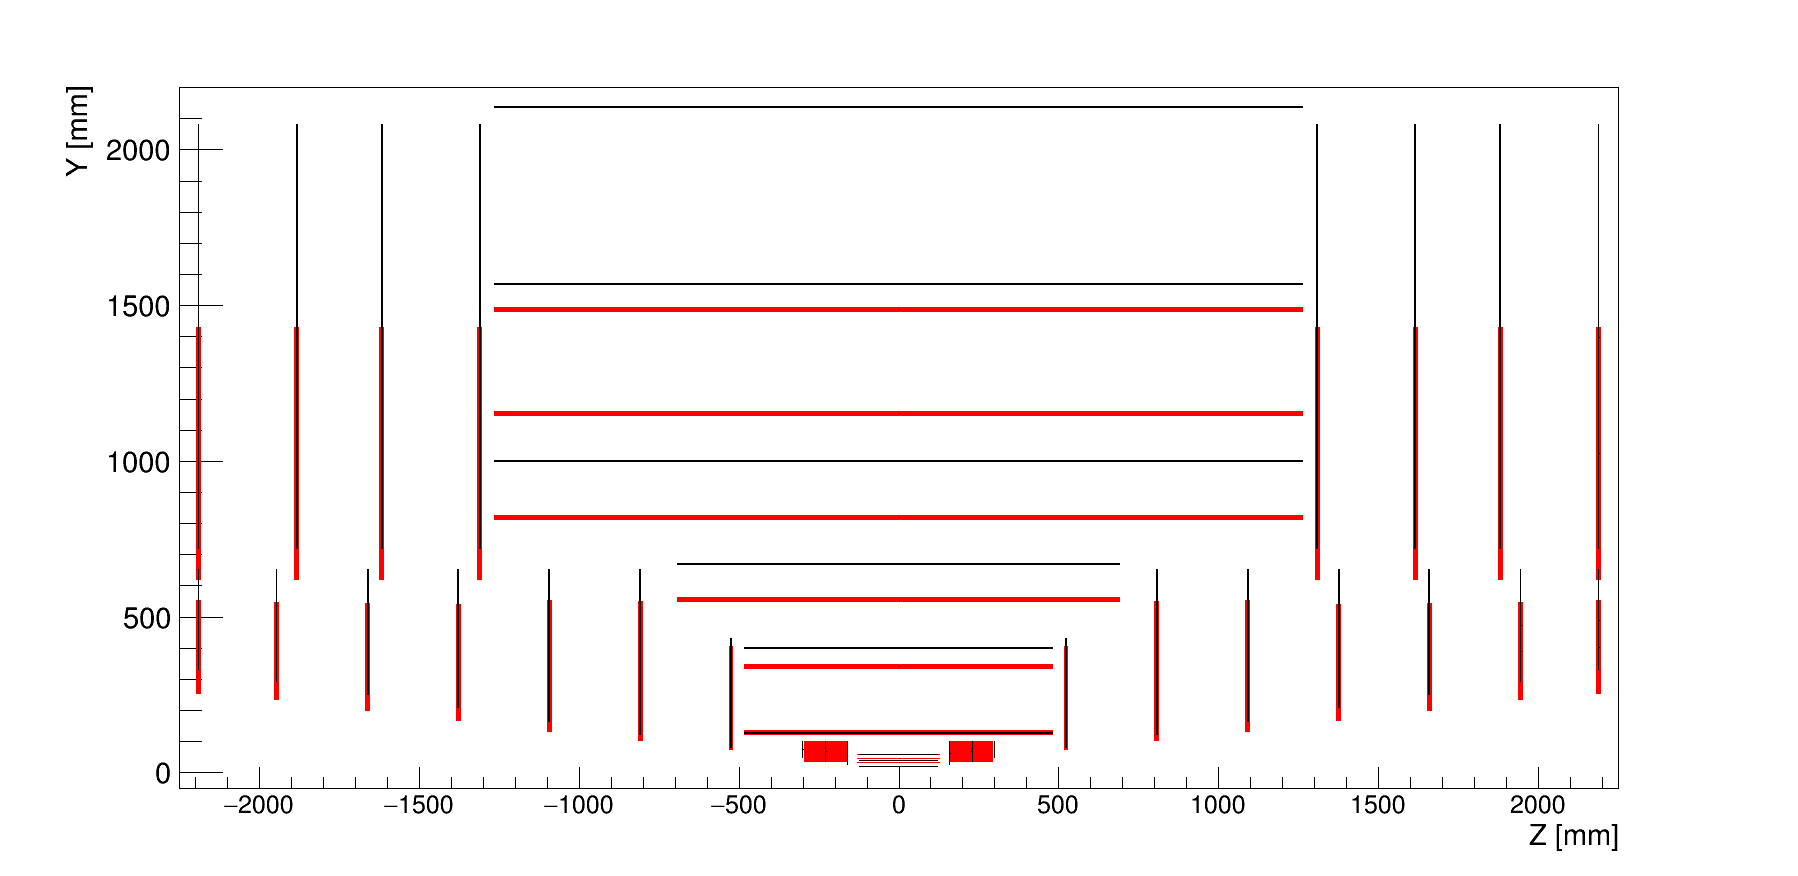
\includegraphics[width=12cm]{CLIC_vs_FCCee_trackingSystem.png}};


 \node[inner sep=0pt] (tmp) at (\xRefPosOne,\yRefPosOne-0.3)
    {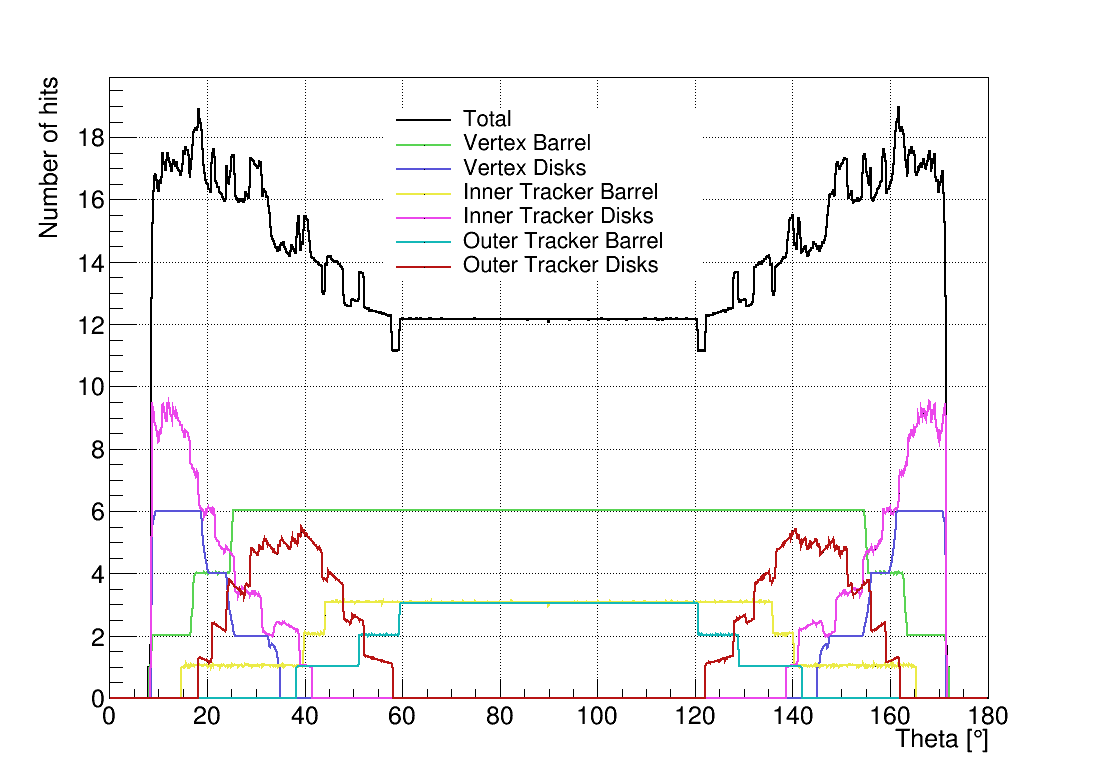
\includegraphics[width=11cm]{FCCee_tracking_coverage_july19.png}};

%     geometryComparison.png
% \node [Box] at (\xRefPosOne+2.5,\yRefPosOne+2) (box){%
%     \begin{minipage}{0.65\textwidth}
% 
%       \begin{itemize}
%         \item The same structure of the Inner and Outer trackers with larger dimentions.
% 	\item Similar coverage of the VTX + Tracker 
%       \end{itemize}
% 
%     \end{minipage}
% };
% \node[fancytitle, right=15pt] at (box.north west) {Transition Radiation Tracker};

\node [Box] at (\xRefPosOne,\yRefPosOne-4.3) (box){%
    \begin{minipage}{0.99\textwidth}

      \begin{itemize}
	\item Tracker coverage (number of sensitive layers as seen from IP). 
	\item More than 12 hits over theta range 8.6$^{\circ}$ - 171.4$^{\circ}$
      \end{itemize}

    \end{minipage}
};

\node [Box] at (\xRefPosOne+2.4,\yRefPosOne+2.5) (box){%
\myCenterBox{FCC-ee}
};

\node [Box] at (\xRefPosOne-2.4,\yRefPosOne+2.5) (box){%
\myVerySmallCenterBox{GEANTINOs}
};

%% HELPER draw advanced helping grid with axises:
% \draw(-0.5,-4) to[grid with coordinates] (11.5,4);
\end{tikzpicture}



 
\end{frame}
%*****************************************************************************

%*****************************************************************************
\begin{frame}{\large \large Material budget of VTX and Tracker}
 
 
 \renewcommand{\yRefPosOne}{0}
\renewcommand{\xRefPosOne}{5.3}
\renewcommand{\xRefIncrementOne}{5.5}
\begin{tikzpicture}[overlay]

 \node[inner sep=0pt] (tmp) at (\xRefPosOne-3,\yRefPosOne-2.5)
    {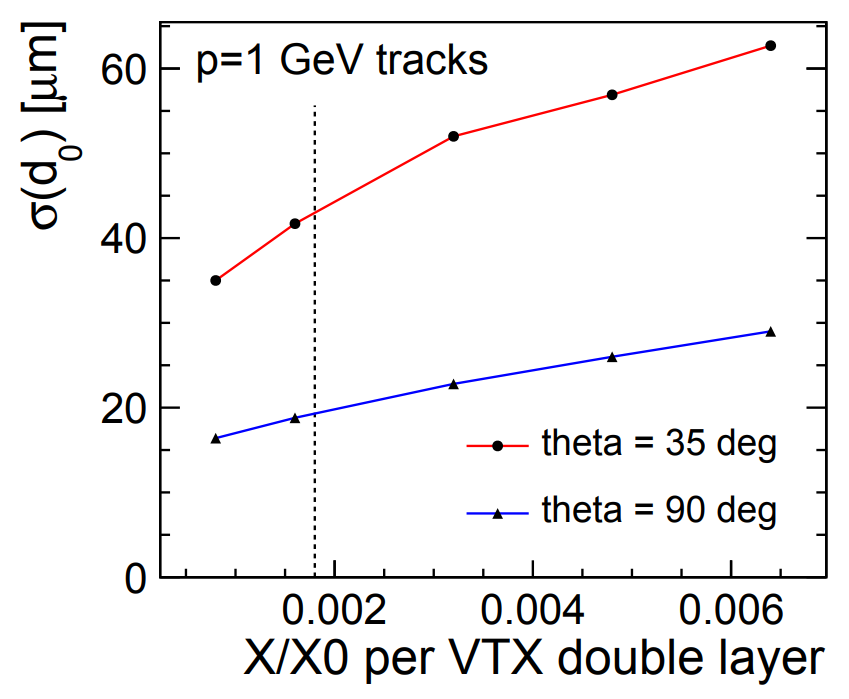
\includegraphics[width=5.5cm]{CLIC_refPlot.png}};

    \node [Box] at (\xRefPosOne-1.5,\yRefPosOne-1.5) (box){%
\myCenterBox{CLIC}
};
    
\node [Box] at (\xRefPosOne,\yRefPosOne+1.5) (box){%
    \begin{minipage}{0.99\textwidth}

  \begin{itemize}
  \item Due to power-pulsing, CLIC VTX can be cooled by air flow. Since power-pulsing is not suitable for FCC-ee operation the material budget of the VTX has to be revised.
  \item The study of the effect of increased material budget in VTX on impact parameter and momentum resolution is ongoing.
%   \item Current model doesn't accomodate support structures and cables... will be added soon
 \end{itemize}

    \end{minipage}
};

\node [Box] at (\xRefPosOne+3,\yRefPosOne-1.5) (box){%
    \begin{minipage}{0.5\textwidth}

  \begin{itemize}
  \item Current FCC-ee model doesn't contain support structures and cables (while it is implemented in CLIC model)... will be added soon
 \end{itemize}

    \end{minipage}
};

% \node[fancytitle, right=15pt] at (box.north west) {Transition Radiation Tracker};

%% HELPER draw advanced helping grid with axises:
% \draw(-0.5,-4) to[grid with coordinates] (11.5,4);
\end{tikzpicture}
 
 
\end{frame}
%*****************************************************************************

%*****************************************************************************
\begin{frame}{\large \large Tracking}

\renewcommand{\yRefPosOne}{0}
\renewcommand{\xRefPosOne}{5.3}
\renewcommand{\xRefIncrementOne}{5.5}
\begin{tikzpicture}[overlay]

 \node[inner sep=0pt] (tmp) at (\xRefPosOne,\yRefPosOne-1.4)
    {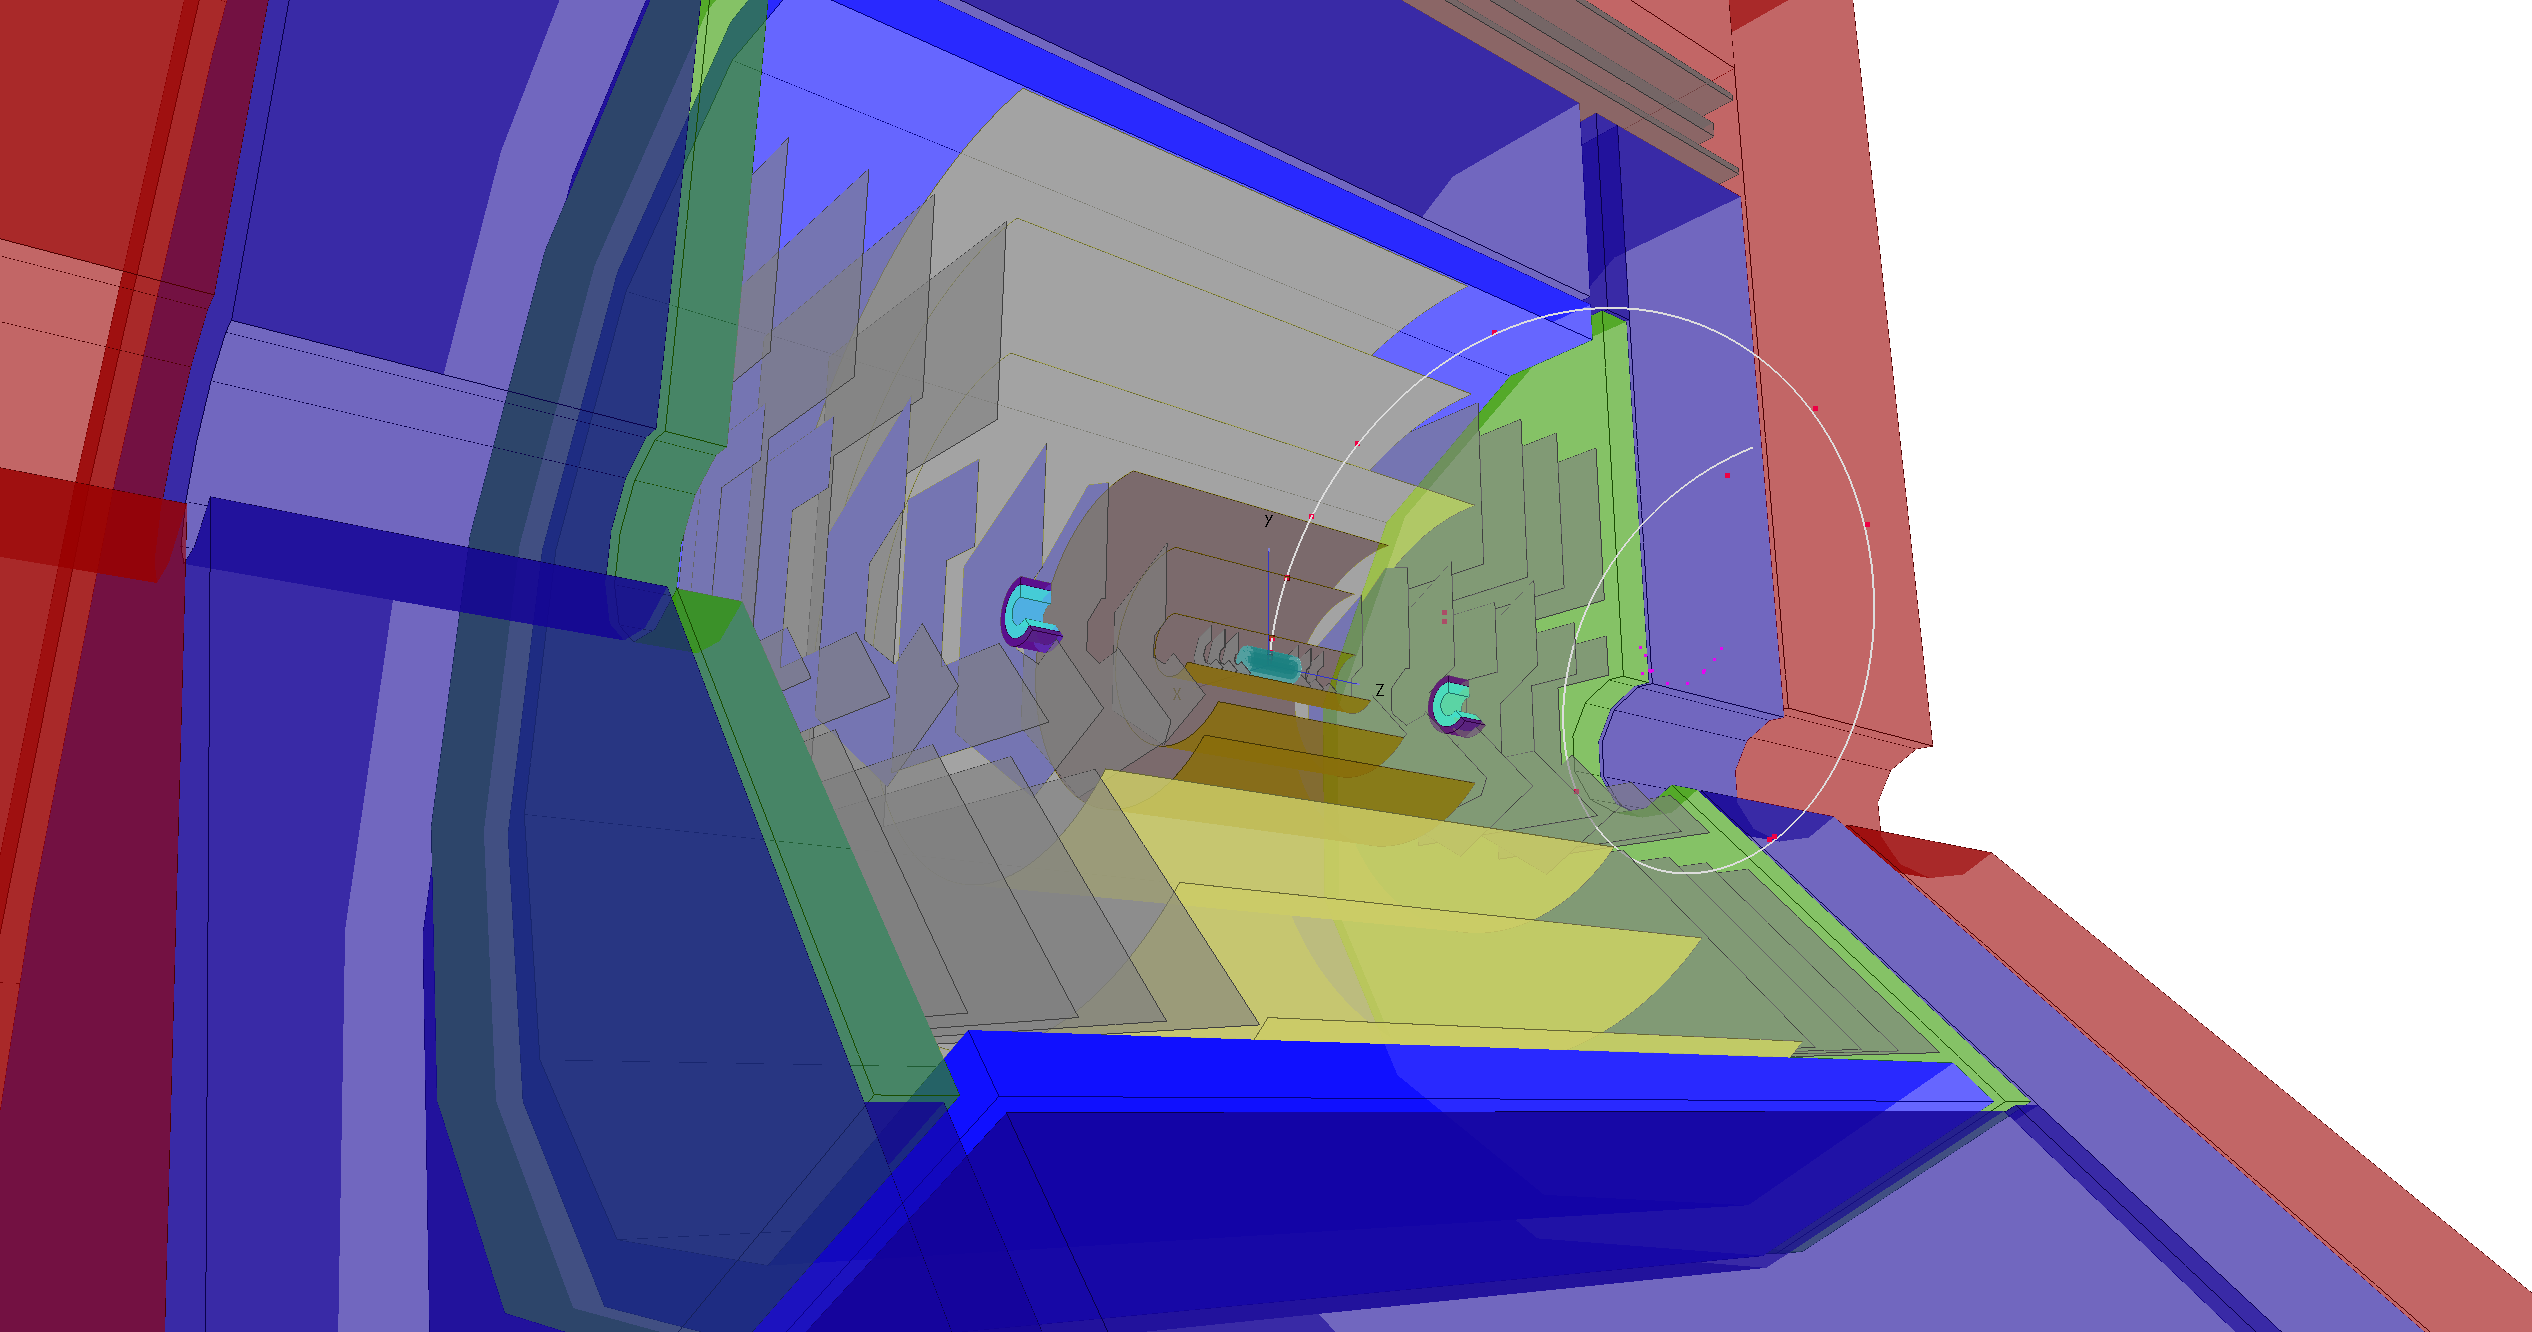
\includegraphics[width=10cm]{eventDisplay/eventDisplay_v1.png}};

    
\node [Box] at (\xRefPosOne,\yRefPosOne+2.57) (box){%
    \begin{minipage}{0.99\textwidth}

  \begin{itemize}
  \item Two tracking algorithms are available: 
  \begin{itemize}
   \item truth tracking - track fitting is done by using all hits produced by particle (by using truth information)
   \item conformal tracking - hits are found by pattern recognition algorithm in conformal space
  \end{itemize}
  \item All results shown below are obtained with truth tracking.
  \item Single-point resolution (sigma): VTX - 3$\times$3 $\mu$m; IT - 7$\times$300$\mu$m; OT - 7$\times$3000$\mu$m
 \end{itemize}

    \end{minipage}
};

\node [Box] at (\xRefPosOne,\yRefPosOne-4.4) (box){%
    \begin{minipage}{0.99\textwidth}

  \begin{itemize}
  \item Charged particles with p$_\mathrm{T} >$ 0.65 GeV reach calorimeter.
 \end{itemize}

    \end{minipage}
};

% \node[fancytitle, right=15pt] at (box.north west) {Transition Radiation Tracker};

\node [Box] at (\xRefPosOne+3.8,\yRefPosOne+0.5) (box){%
\myCenterBox{FCC-ee}
};


%% HELPER draw advanced helping grid with axises:
% \draw(-0.5,-4) to[grid with coordinates] (11.5,4);
\end{tikzpicture}

 
 


 
\end{frame}
%*****************************************************************************

%*****************************************************************************
\begin{frame}{\large \large Momentum resolution}

\renewcommand{\yRefPosOne}{0}
\renewcommand{\xRefPosOne}{5.3}
\renewcommand{\xRefIncrementOne}{5.5}
\begin{tikzpicture}[overlay]

 \node[inner sep=0pt] (tmp) at (\xRefPosOne,\yRefPosOne-0.5)
    {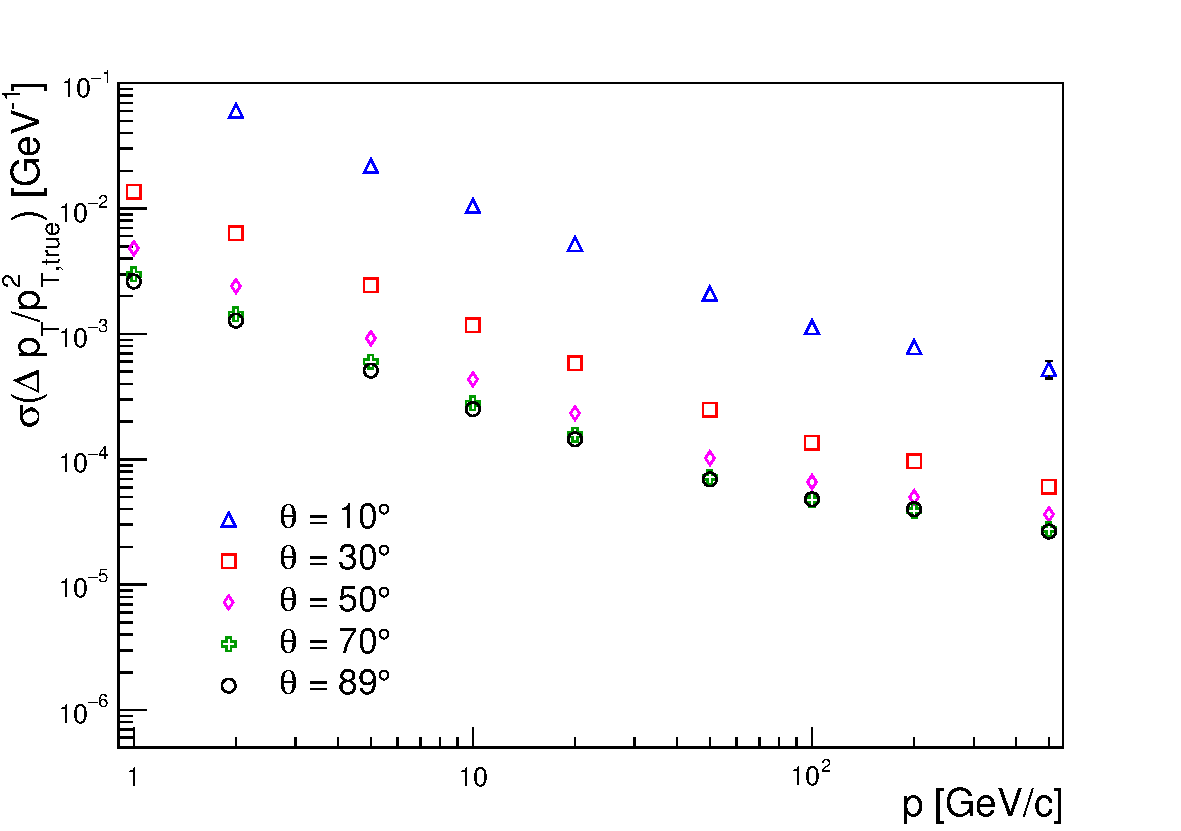
\includegraphics[width=11.5cm]{EmiliaPlots_July30/momRes_v2.pdf}};

    
\node [mybox] at (\xRefPosOne+2,\yRefPosOne-2.6) (box){
    \begin{minipage}{0.34\textwidth}

    $\sigma_{\mathrm{p_T}}/ \mathrm{p_T}^2 \simeq$ 4.8 $\cdot$ 10$^{-5}$ GeV$^{-1}$ \\ \vspace{0.01cm} \\ at p = 100 GeV at 89$^{\circ}$
    
%       \begin{itemize}
% 	\item $\sigma_{\mathrm{p_T}}/ \mathrm{p_T}^2 \simeq$ 4.8 $\cdot$ 10$^{-5}$ GeV$^{-1}$ \\at p$_\mathrm{T}$ = 100 GeV at 90$^{\circ}$
%       \end{itemize}

    \end{minipage}
};
% \node[fancytitle, right=15pt] at (box.north west) {Transition Radiation Tracker};

\node [Box] at (\xRefPosOne+3,\yRefPosOne+2.5) (box){%
\myCenterBox{FCC-ee}
};
\node [Box] at (\xRefPosOne+3,\yRefPosOne+2.1) (box){%
\myCenterBox{full simulation}
};

\node [Box] at (\xRefPosOne,\yRefPosOne-4.65) (box){%
    \begin{minipage}{0.99\textwidth}

  \begin{itemize}
  \item Resolution was simulated with muons generated by particle gun
 \end{itemize}

    \end{minipage}
};

%% HELPER draw advanced helping grid with axises:
% \draw(-0.5,-4) to[grid with coordinates] (11.5,4);
\end{tikzpicture}
 
\end{frame}
%*****************************************************************************
%*****************************************************************************
\begin{frame}{\large \large Number of hits per track}
 
\renewcommand{\yRefPosOne}{0}
\renewcommand{\xRefPosOne}{5.3}
\renewcommand{\xRefIncrementOne}{5.5}
\begin{tikzpicture}[overlay]

 \node[inner sep=0pt] (tmp) at (\xRefPosOne-3,\yRefPosOne+1.4)
    {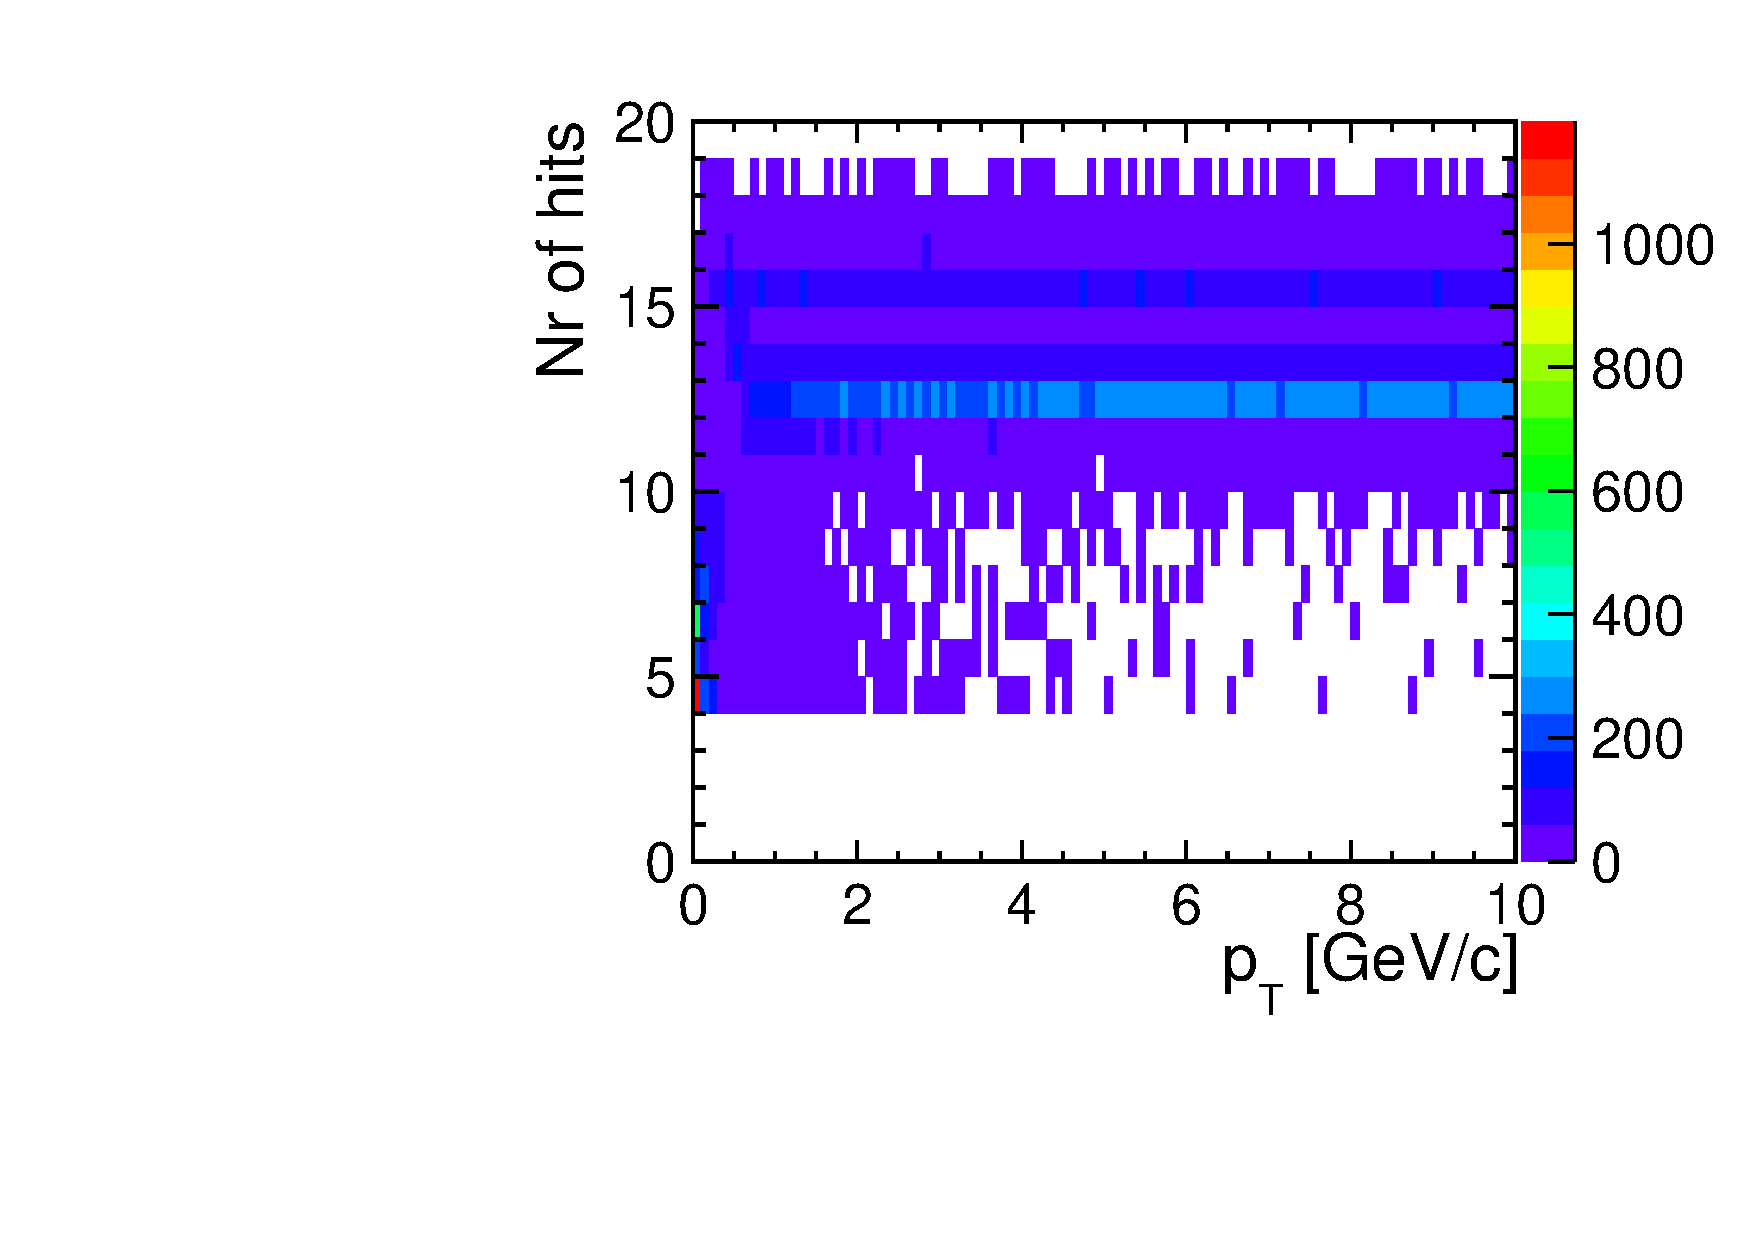
\includegraphics[width=5cm]{EmiliaPlots_July30/UPDATED_FCCo5v03_Nhits_pt.pdf}};

 \node[inner sep=0pt] (tmp) at (\xRefPosOne+3,\yRefPosOne+1.4)
    {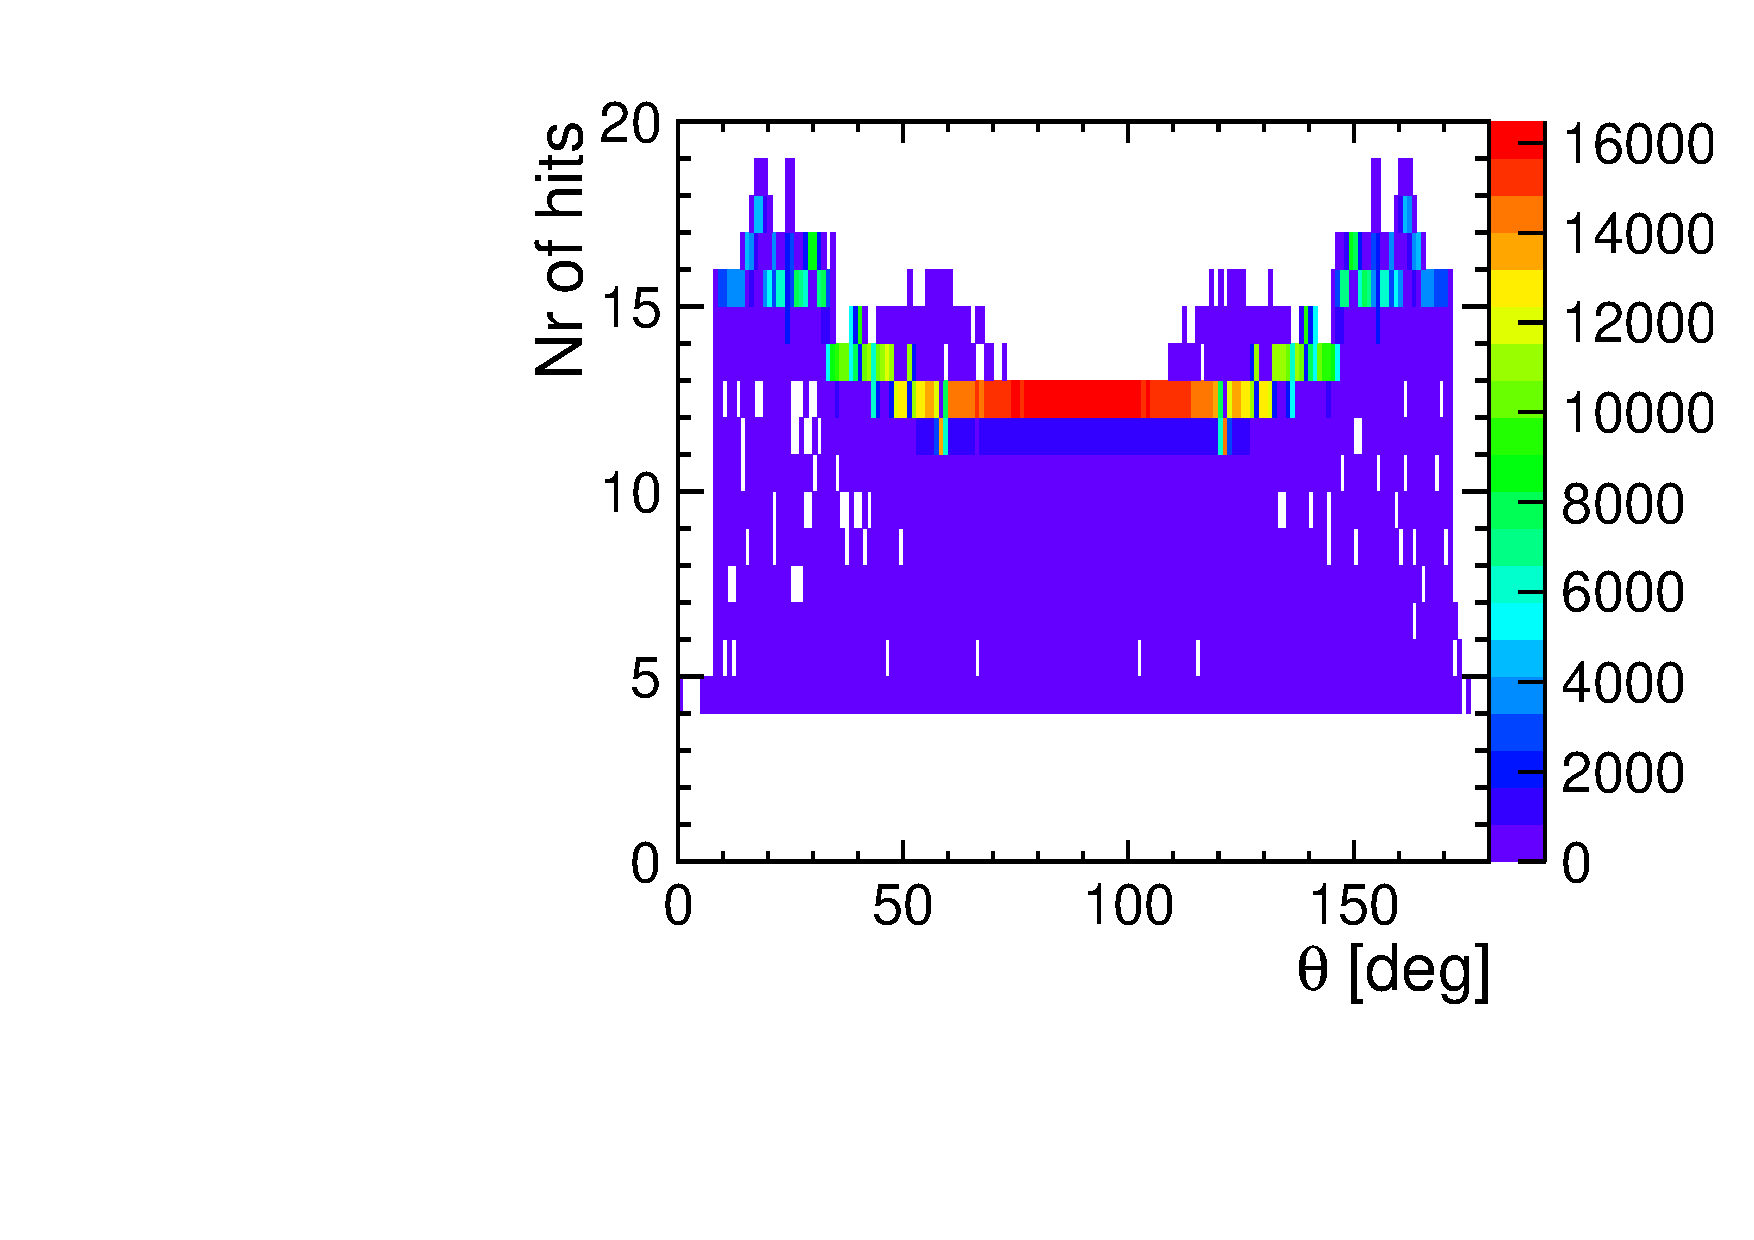
\includegraphics[width=5cm]{EmiliaPlots_July30/UPDATED_FCCo5v03_Nhits_theta.pdf}};
  
 \node[inner sep=0pt] (tmp) at (\xRefPosOne-3,\yRefPosOne-2.8)
    {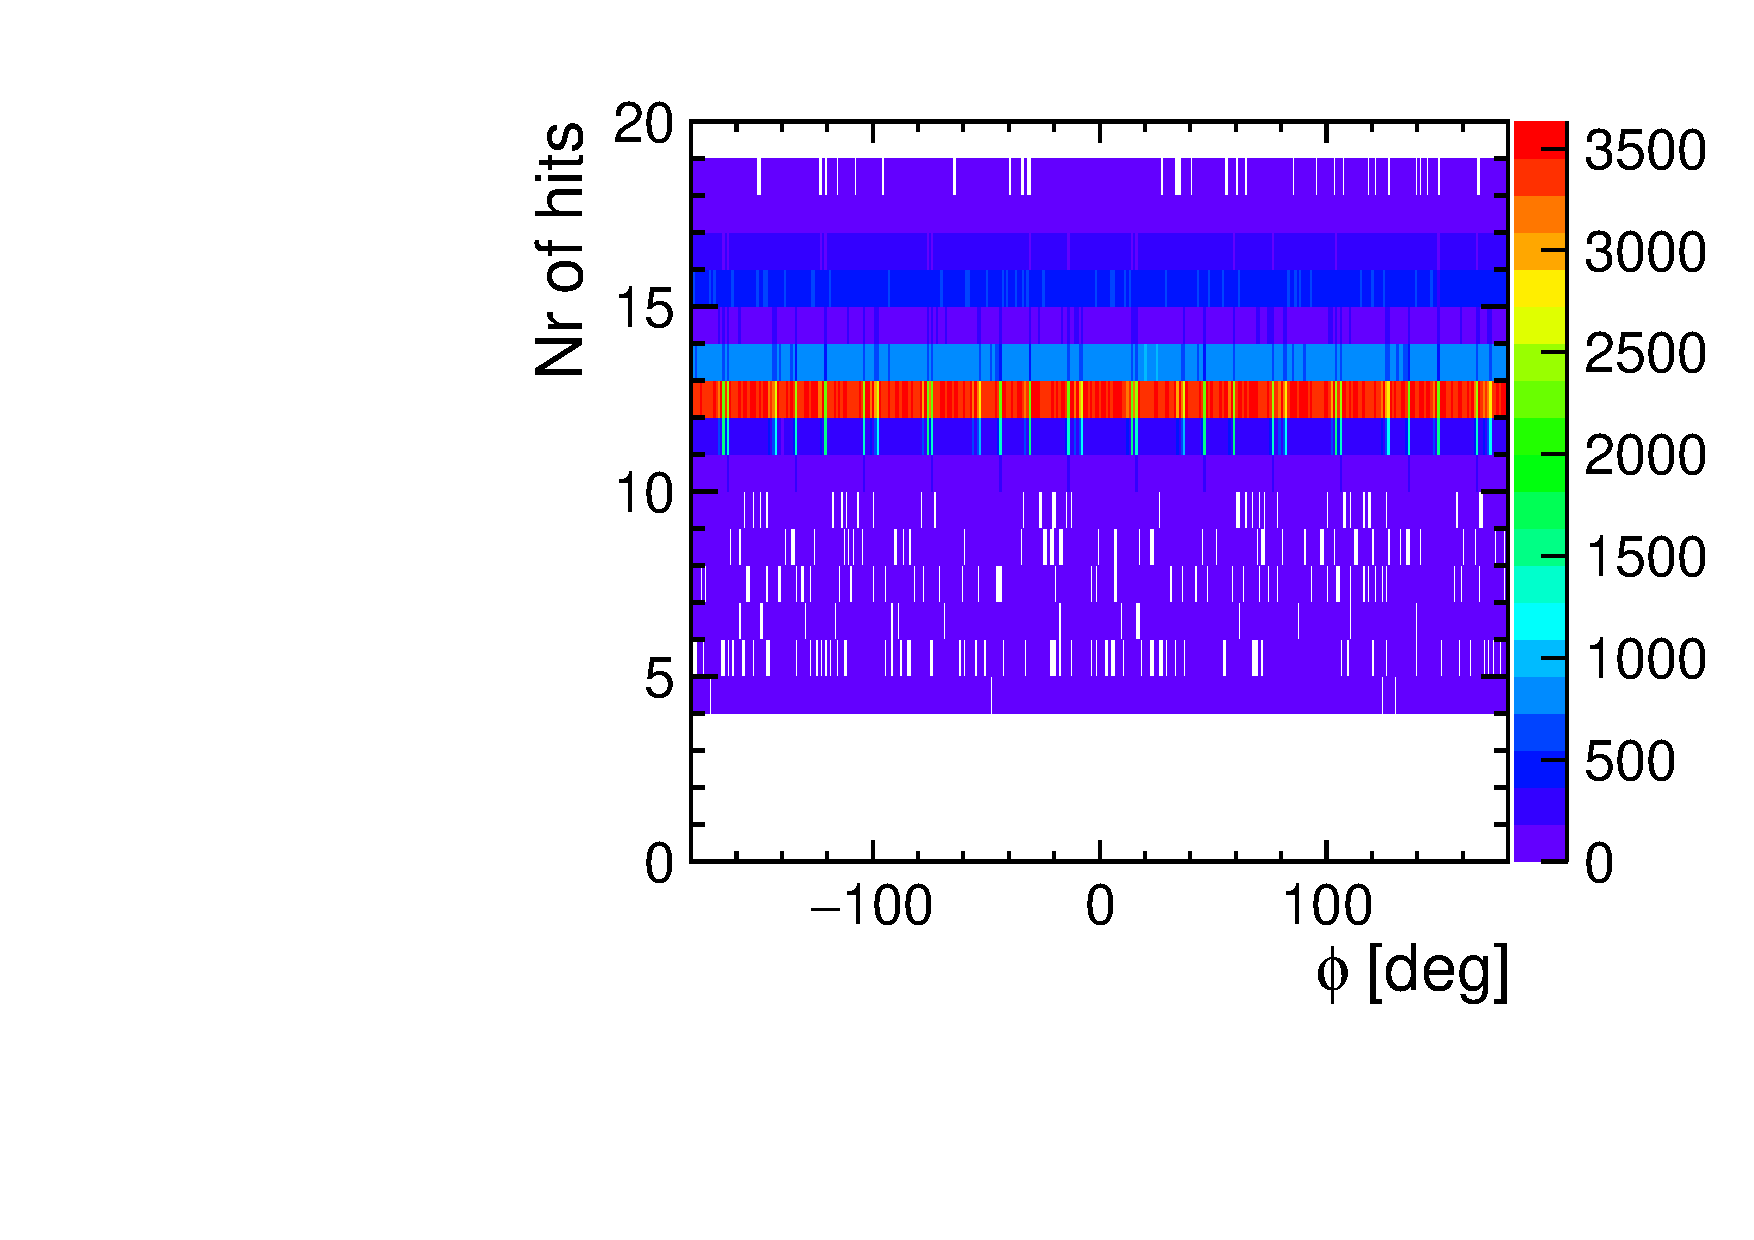
\includegraphics[width=5cm]{EmiliaPlots_July30/UPDATED_FCCo5v03_Nhits_phi.pdf}};
    
\node [Box] at (\xRefPosOne+3,\yRefPosOne-2.5) (box){%
    \begin{minipage}{0.5\textwidth}

  \begin{itemize}
  \item Muons are generated with general particle source with: 
  \begin{itemize}
   \item isotropic angular distribution \\ (uniform in cos($\theta$))
   \item uniform energy distribution
  \end{itemize}
  \item 12 hits per track on average \\ $\to$ all hits are used during track fitting
 \end{itemize}

    \end{minipage}
};
    
% \node [Box] at (\xRefPosOne+3.5,\yRefPosOne-2.5) (box){%
%   \begin{minipage}{0.5\textwidth}
%     \begin{itemize}
%       \item Number of hits per track as function of p$_\mathrm{T}$, Theta and Phi  
%     \end{itemize}
%   \end{minipage}
% };
% \node[fancytitle, right=15pt] at (box.north west) {Transition Radiation Tracker};

%% HELPER draw advanced helping grid with axises:
% \draw(-0.5,-4) to[grid with coordinates] (11.5,4);
\end{tikzpicture}
 
\end{frame}
%*****************************************************************************

%*****************************************************************************
\begin{frame}{\large \large Tracking efficiency as function of p$_\mathrm{T}$}
 

\renewcommand{\yRefPosOne}{0}
\renewcommand{\xRefPosOne}{5.3}
\renewcommand{\xRefIncrementOne}{5.5}
\begin{tikzpicture}[overlay]

 \node[inner sep=0pt] (tmp) at (\xRefPosOne-3,\yRefPosOne+1.4)
    {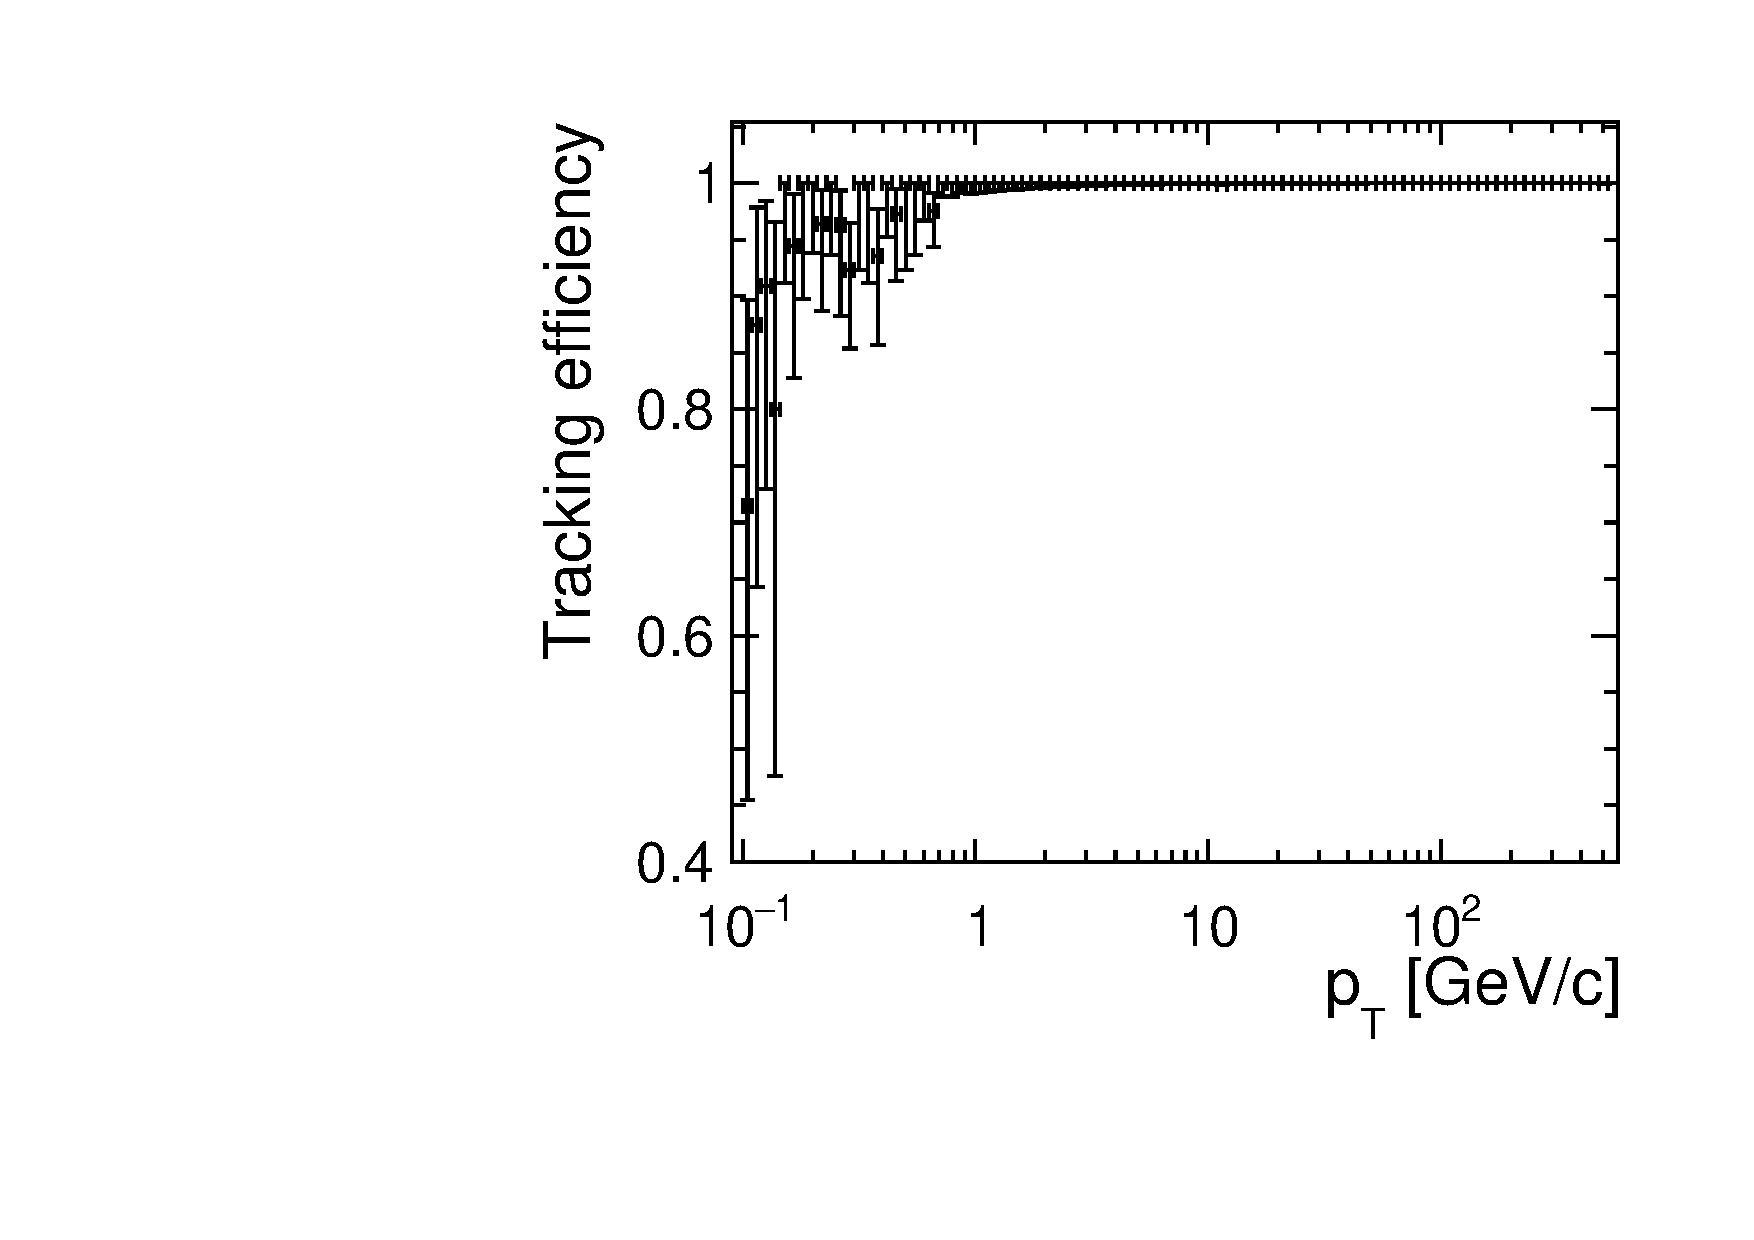
\includegraphics[width=5cm]{EmiliaPlots_July30/UPDATED_FCCo5v03_eff_pt.pdf}};

 \node[inner sep=0pt] (tmp) at (\xRefPosOne+3,\yRefPosOne+1.4)
    {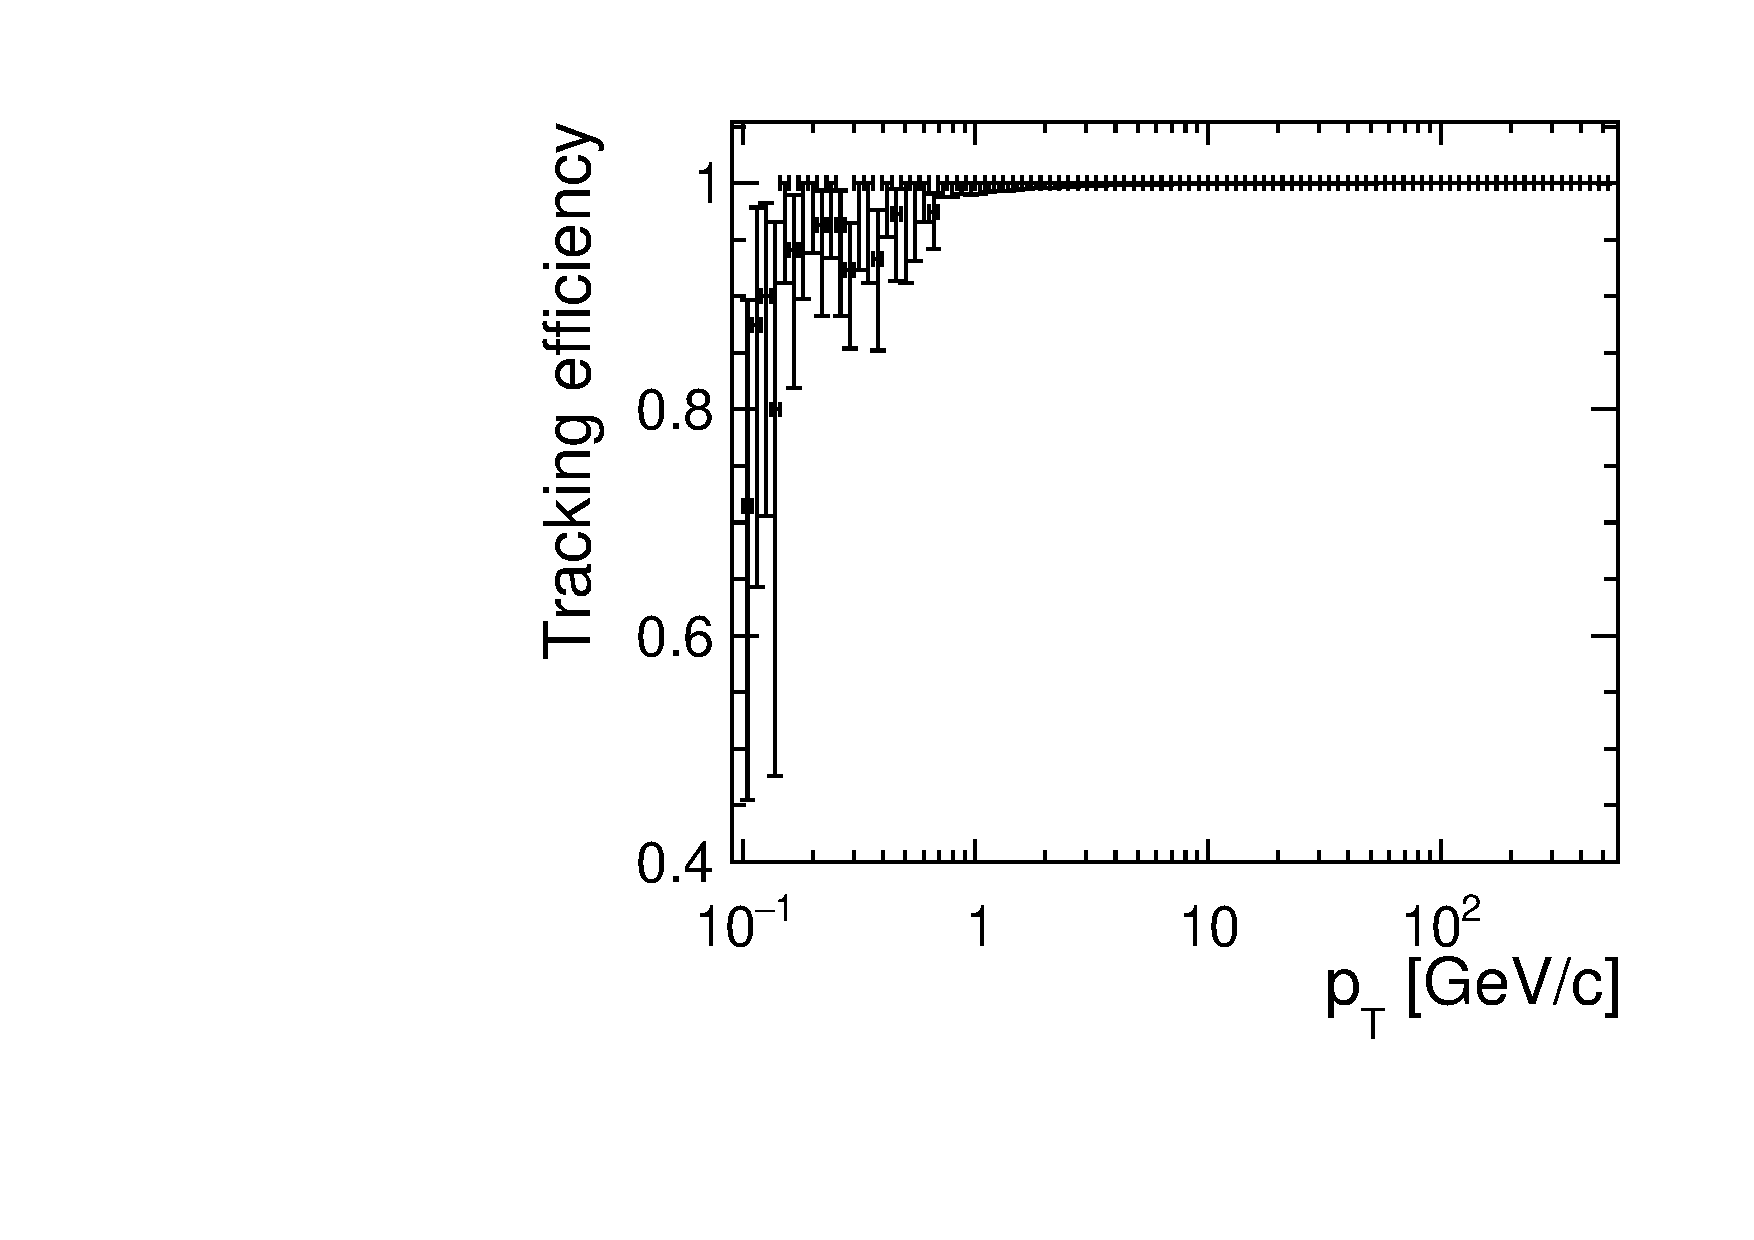
\includegraphics[width=5cm]{EmiliaPlots_July30/UPDATED_FCCo5v03_eff_pt_withCuts.pdf}};
      
      
\node [PixelBox] at (\xRefPosOne-3,\yRefPosOne-2.2) (box){%
  \begin{minipage}{0.43\textwidth}
Tracking efficiency = $\dfrac{N^{reconstructed}_{tracks}}{N^{reconstructable}_{particles}}$
  \end{minipage}
};
      
\node [Box] at (\xRefPosOne+3,\yRefPosOne-2.5) (box){%
  \begin{minipage}{0.5\textwidth}
    \begin{itemize}
      \item reconstructable particles:
      \begin{itemize}
       \item PDG ID = 13 (muon)
       \item N$_{hits} \geqslant$ 4
       \item $|$cos$(\theta)| <$ 0.99
       \item p$_\mathrm{T} \geqslant$ 0.1 GeV/c
%        \item dist from IP < 10 cm
       \item particle track is not a loop \\(does not have two hits on the same layer of the same subdetector)
      \end{itemize}

    \end{itemize}
  \end{minipage}
};
% \node[fancytitle, right=15pt] at (box.north west) {Transition Radiation Tracker};

\node [Box] at (\xRefPosOne+3.3,\yRefPosOne+0.4) (box){%
\myCenterBox{15 $< \theta <$ 165}
};

%% HELPER draw advanced helping grid with axises:
% \draw(-0.5,-4) to[grid with coordinates] (11.5,4);
\end{tikzpicture}
 
\end{frame}
%*****************************************************************************

%*****************************************************************************
\begin{frame}{\large \large Tracking efficiency as function of $\theta$ and $\phi$}
 
\renewcommand{\yRefPosOne}{0}
\renewcommand{\xRefPosOne}{5.3}
\renewcommand{\xRefIncrementOne}{5.5}
\begin{tikzpicture}[overlay]

 \node[inner sep=0pt] (tmp) at (\xRefPosOne-3,\yRefPosOne+1.4)
    {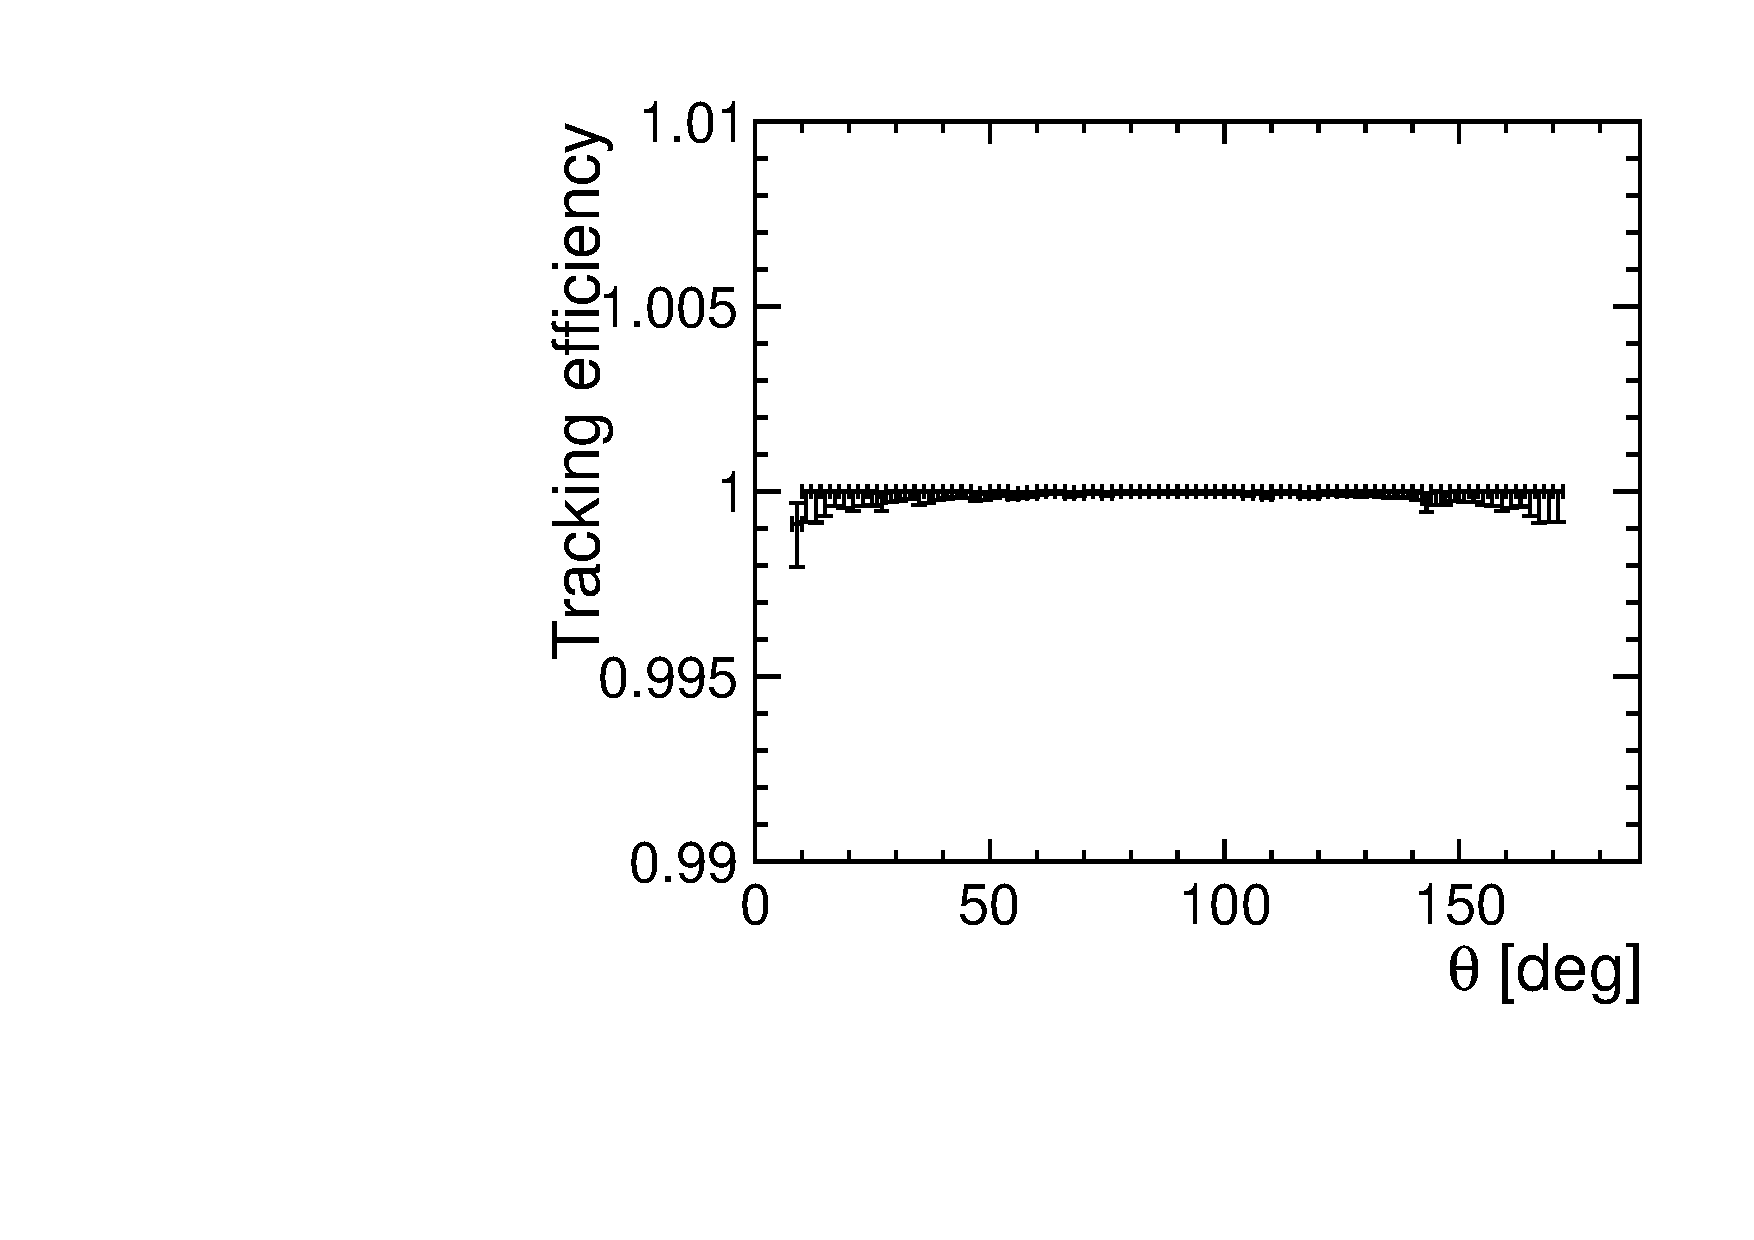
\includegraphics[width=5cm]{EmiliaPlots_July30/UPDATED_FCCo5v03_eff_theta.pdf}};

 \node[inner sep=0pt] (tmp) at (\xRefPosOne+3,\yRefPosOne+1.4)
    {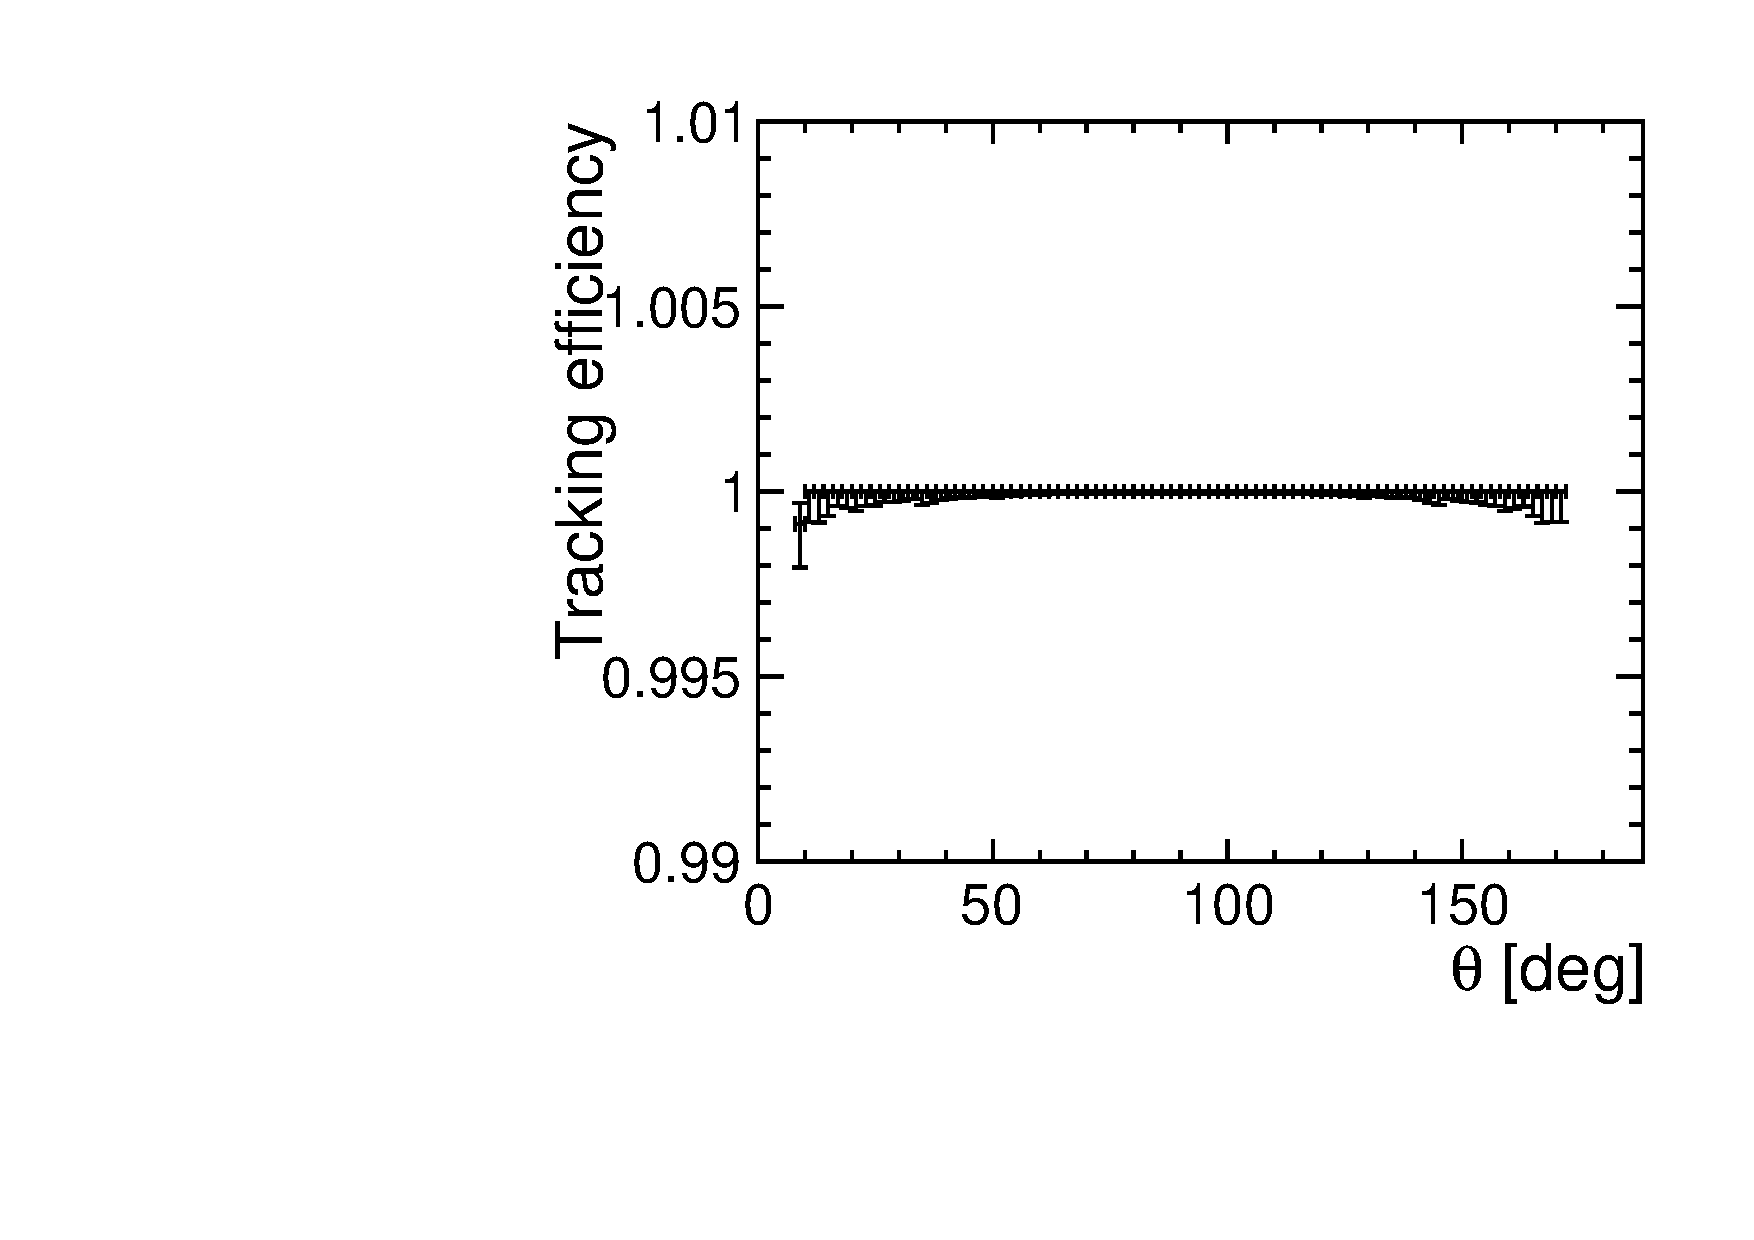
\includegraphics[width=5cm]{EmiliaPlots_July30/UPDATED_FCCo5v03_eff_theta_withCuts.pdf}};
  
 \node[inner sep=0pt] (tmp) at (\xRefPosOne-3,\yRefPosOne-2.8)
    {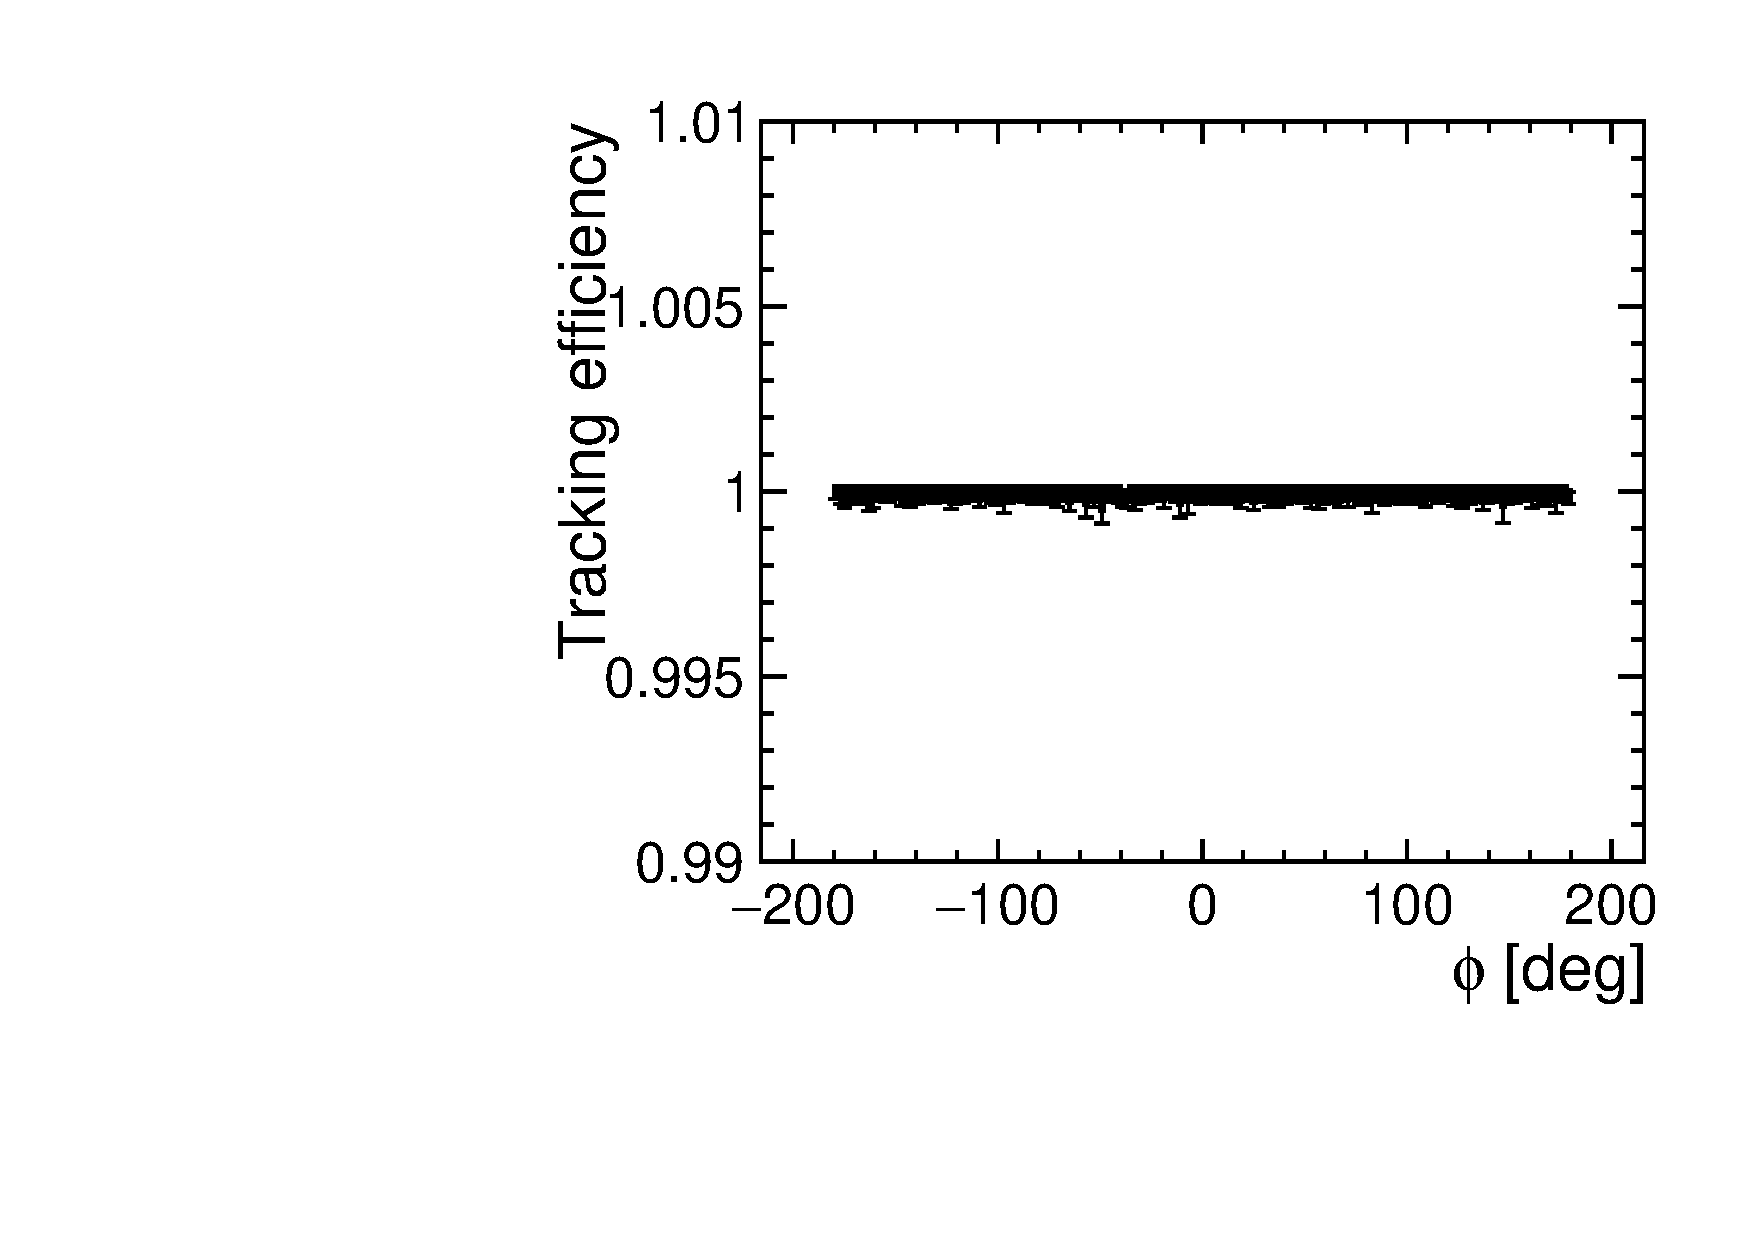
\includegraphics[width=5cm]{EmiliaPlots_July30/UPDATED_FCCo5v03_eff_phi.pdf}};

 \node[inner sep=0pt] (tmp) at (\xRefPosOne+3,\yRefPosOne-2.8)
    {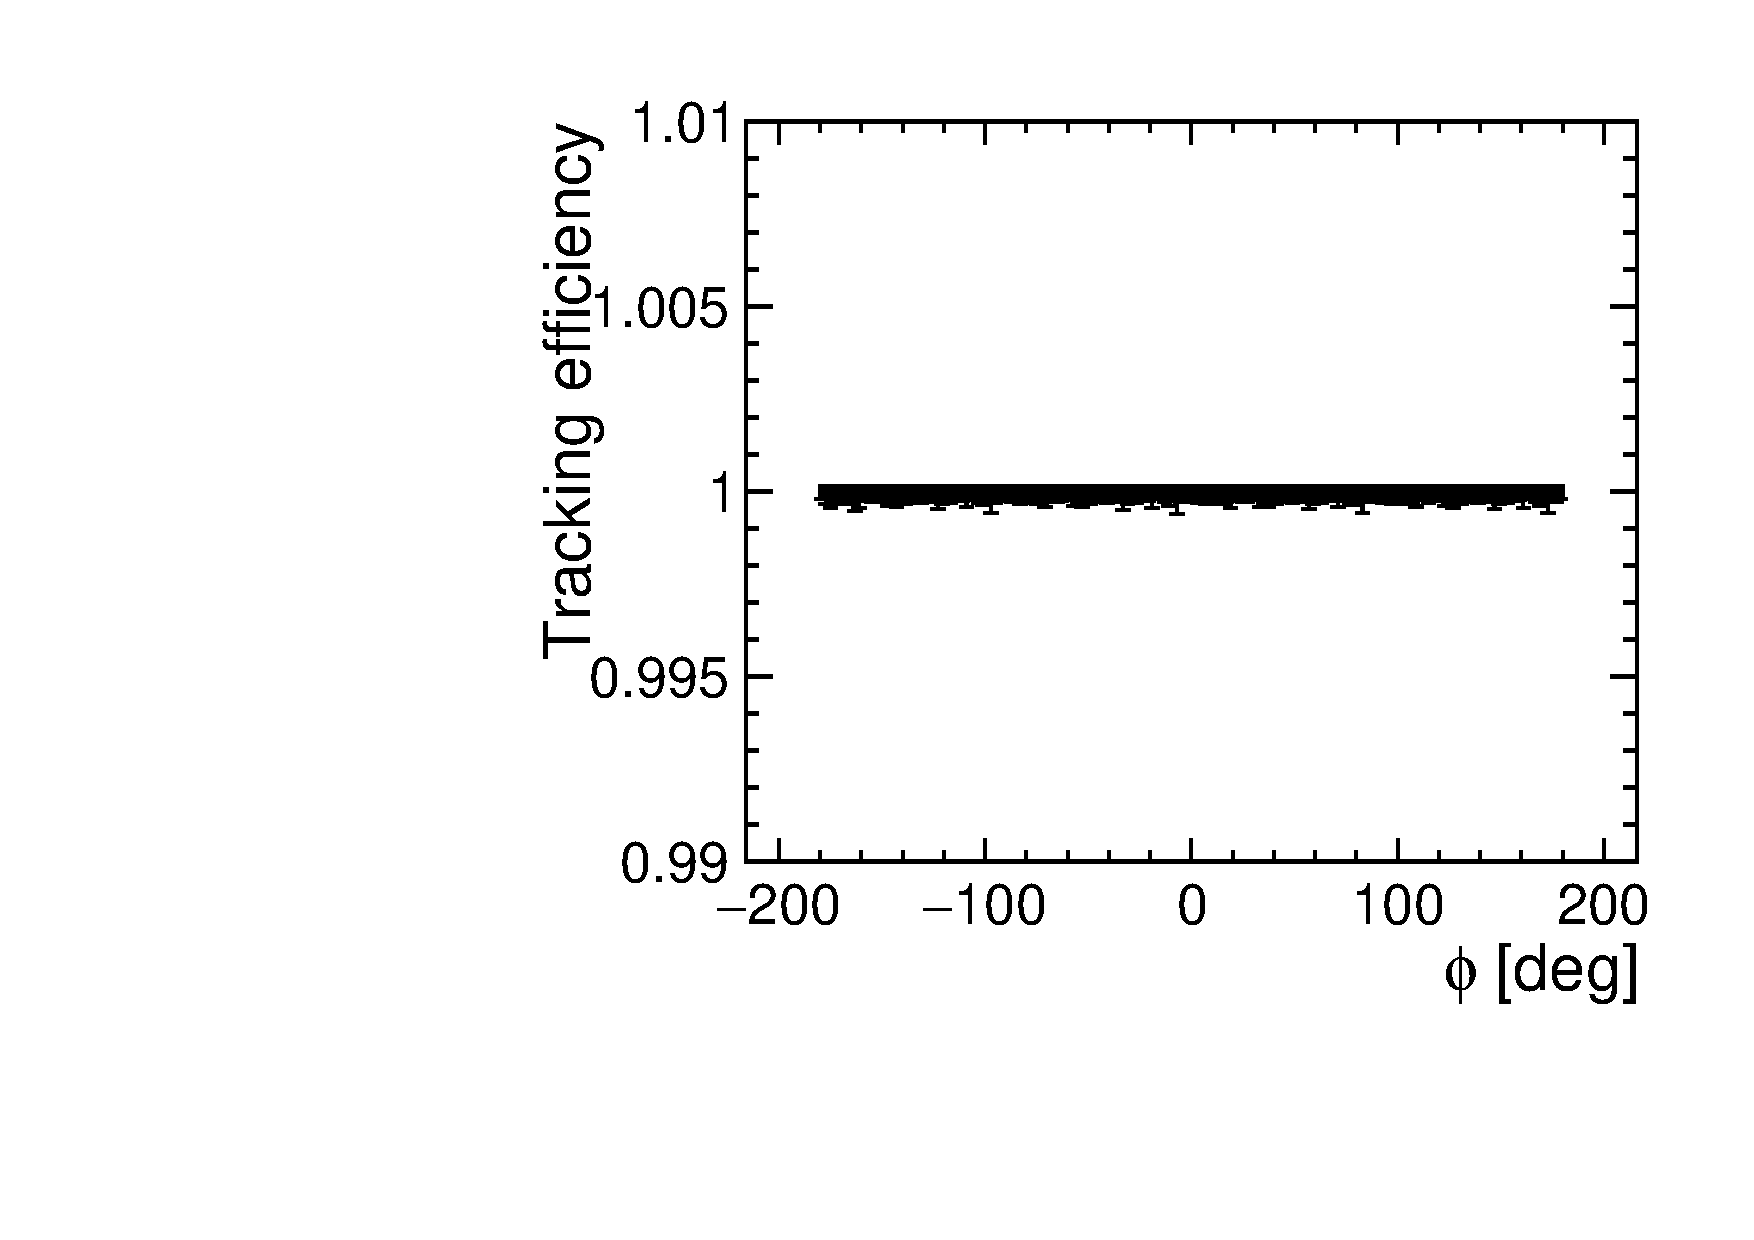
\includegraphics[width=5cm]{EmiliaPlots_July30/UPDATED_FCCo5v03_eff_phi_withCuts.pdf}};
    
\node [Box] at (\xRefPosOne+3.3,\yRefPosOne+2.8) (box){%
\myCenterBox{p$_\mathrm{T} >$ 1 GeV}
};

\node [Box] at (\xRefPosOne+3.3,\yRefPosOne-1.4) (box){%
\myCenterBox{p$_\mathrm{T} >$ 1 GeV}
};
    
%% HELPER draw advanced helping grid with axises:
% \draw(-0.5,-4) to[grid with coordinates] (11.5,4);
\end{tikzpicture}

 
\end{frame}
%*****************************************************************************

%*****************************************************************************
\begin{frame}{\large \large Summary and outlook}
 
 
 
 
 \renewcommand{\yRefPosOne}{0}
\renewcommand{\xRefPosOne}{5.3}
\renewcommand{\xRefIncrementOne}{5.5}
\begin{tikzpicture}[overlay]

      
\node [Box] at (\xRefPosOne,\yRefPosOne+2) (box){%
  \begin{minipage}{0.99\textwidth}
 \begin{itemize}
  \item Complete FCC-ee detector model is available for performance studies
  \item Tracking performance was studied with full simulation and reconstruction (truth tracking)
    \end{itemize}
  \end{minipage}
};
% \node[fancytitle, right=15pt] at (box.north west) {Transition Radiation Tracker};


\node [PixelBox] at (\xRefPosOne,\yRefPosOne-2) (box){%
  \begin{minipage}{0.99\textwidth}
 \begin{itemize}
     \item Conformal tracking performance (presently being completed for CLIC)
     \item Conformal tracking for complex events (e.g. Z $\to$ uds events)
     \item Conformal tracking with overlay of beam background \\[0.3cm]

     \item Effect of increased material budget in VTX \\[0.3cm]
     
     \item Calorimeter studies: 
     \begin{itemize}
      \item single electrons, photons, muons and pions \\
	    (PID efficiency as function of pT and theta)
      \item complex events - PID efficiency
      \item jet energy resolution
      \item all above with beam background overlaid
     \end{itemize}

%      electron and photon PID efficiencies using the Pandora Particle Flow Algorithm, jets performance
    \end{itemize}
  \end{minipage}
};

\node [Box] at (\xRefPosOne-4.2,\yRefPosOne+0.4) (box){%
\myCenterBox[PixelColor]{Next steps}
};

% \node[fancytitle, right=15pt] at (box.north west) {Next steps};
% \node[fancytitle, right=15pt] at (box.north west) {LUCID};

\end{tikzpicture}
  
\end{frame}
%*****************************************************************************

%------------------------------------------------
\begin{frame}
\frametitle{BACKUP} 
 
\end{frame}
%------------------------------------------------

%------------------------------------------------
\begin{frame}
\frametitle{VTX barrel layout} 

\renewcommand{\yRefPosOne}{0}
\renewcommand{\xRefPosOne}{5.3}
\renewcommand{\xRefIncrementOne}{5}
\begin{tikzpicture}[overlay]

 \node[inner sep=0pt] (tmp) at (\xRefPosOne,\yRefPosOne-0.8)
    {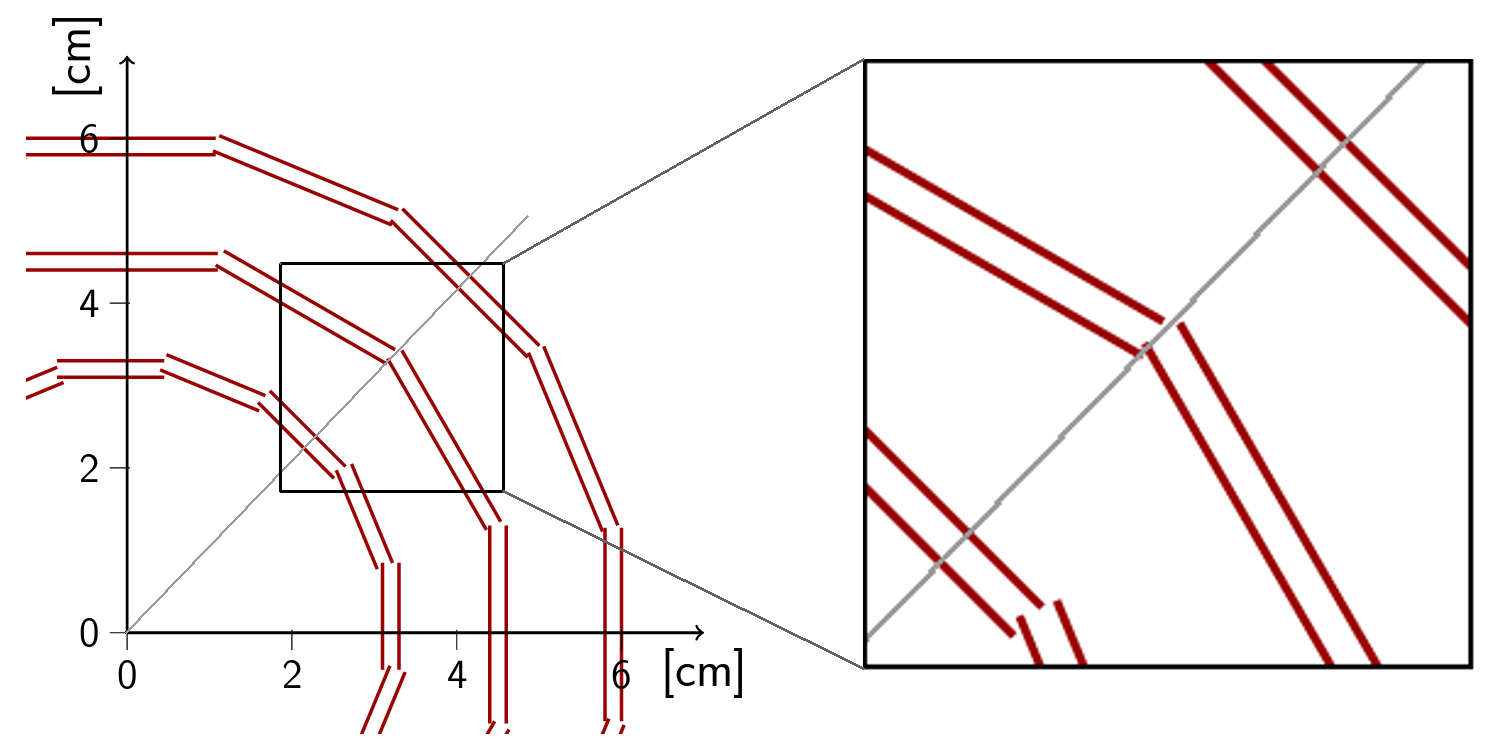
\includegraphics[width=11.5cm]{VTX_layout_hole_explanation_v3.png}};

\node [Box] at (\xRefPosOne-3.5,\yRefPosOne+1.5) (box){%
\myCenterBox{CLIC}
};
    
\end{tikzpicture}

    
\end{frame}
%------------------------------------------------

%------------------------------------------------
\begin{frame}
\frametitle{Photon energy resolution for different number of ECAL layers} 


\renewcommand{\yRefPosOne}{0}
\renewcommand{\xRefPosOne}{5.3}
\renewcommand{\xRefIncrementOne}{5}
\begin{tikzpicture}[overlay]

 \node[inner sep=0pt] (tmp) at (\xRefPosOne,\yRefPosOne-0.8)
    {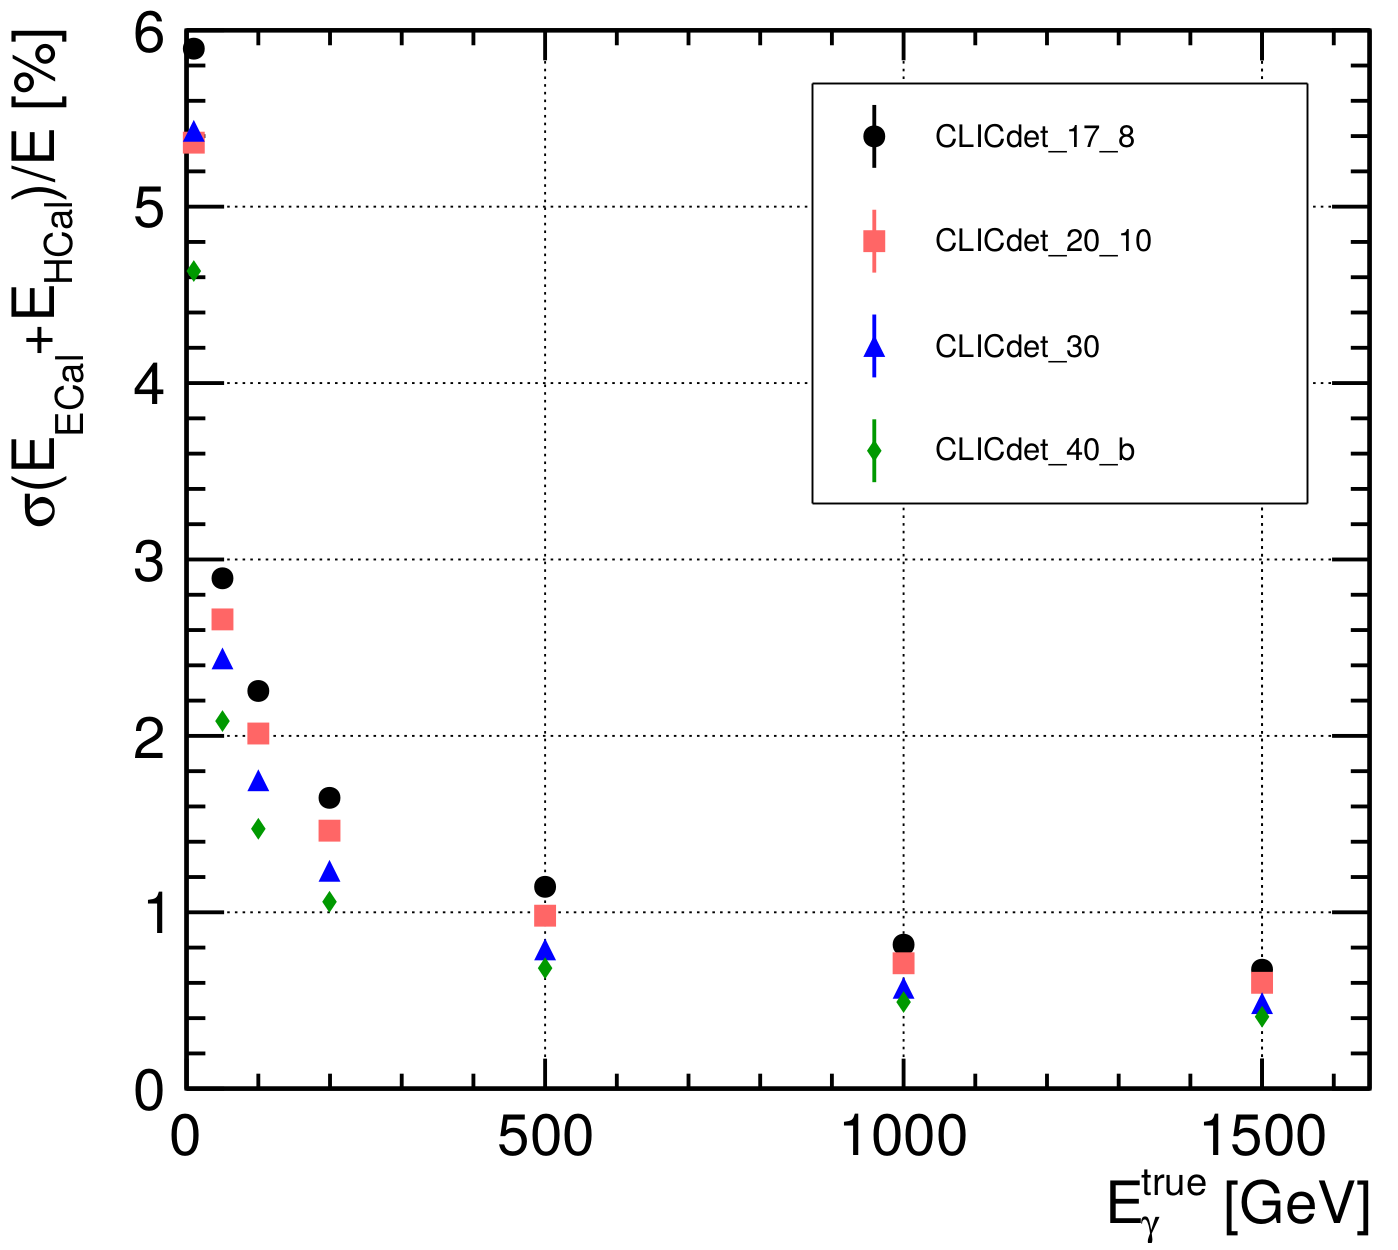
\includegraphics[width=9cm]{ECAL_res.png}};

\node [Box] at (\xRefPosOne-2,\yRefPosOne+2.5) (box){%
\myCenterBox{CLIC}
};
    
\end{tikzpicture}


    
\end{frame}
%------------------------------------------------


\end{document}

